\documentclass{article}
\usepackage{neurips_2026}
\usepackage[utf8]{inputenc}
\usepackage[T1]{fontenc}
\usepackage{hyperref}
\usepackage{url}
\usepackage{booktabs}
\usepackage{amsfonts,amsmath,amssymb}
\usepackage{nicefrac}
\usepackage{microtype}
\usepackage{xcolor}
\usepackage{graphicx}
\usepackage{placeins}

% generated by quoted_numbers.py from ../results; do not edit
\newcommand{\nVerified}{1781}
\newcommand{\nClaims}{1781}
\newcommand{\nExactTie}{54}
\newcommand{\nSeasons}{69}
\newcommand{\ArenaConeB}{3}
\newcommand{\ArenaConeFrac}{0.01\%}
\newcommand{\ArenaConeZ}{0.2}
\newcommand{\ArenaConeLev}{29}
\newcommand{\ArenaN}{57477}
\newcommand{\ArenaCtwoMed}{7}
\newcommand{\ArenaCtwoMin}{1}
\newcommand{\ArenaCtwoMax}{222}
\newcommand{\ArenaCtwoFracMed}{0.012\%}
\newcommand{\ArenaCtwoZMed}{0.2}
\newcommand{\ArenaCtwoLowZ}{16}
\newcommand{\ArenaCtwoCount}{19}
\newcommand{\ArenaCtwoLowZBudMax}{43}
\newcommand{\ArenaLev}{28}
\newcommand{\MTHConeB}{91}
\newcommand{\MTHConeFrac}{2.71\%}
\newcommand{\MTHConeZ}{4.9}
\newcommand{\MTHConeLev}{29}
\newcommand{\MTHN}{3355}
\newcommand{\MTHCtwoMed}{141}
\newcommand{\MTHCtwoMin}{13}
\newcommand{\MTHCtwoMax}{229}
\newcommand{\MTHCtwoFracMed}{4.203\%}
\newcommand{\MTHCtwoZMed}{7.9}
\newcommand{\MTHCtwoLowZ}{1}
\newcommand{\MTHCtwoCount}{5}
\newcommand{\MTHCtwoLowZBudMax}{13}
\newcommand{\MTHLev}{36}
\newcommand{\MTGConeB}{144}
\newcommand{\MTGConeFrac}{6.00\%}
\newcommand{\MTGConeZ}{8.9}
\newcommand{\MTGConeLev}{35}
\newcommand{\MTGN}{2400}
\newcommand{\MTGCtwoMed}{144}
\newcommand{\MTGCtwoMin}{82}
\newcommand{\MTGCtwoMax}{226}
\newcommand{\MTGCtwoFracMed}{6.000\%}
\newcommand{\MTGCtwoZMed}{8.9}
\newcommand{\MTGCtwoLowZ}{0}
\newcommand{\MTGCtwoCount}{5}
\newcommand{\MTGCtwoLowZBudMax}{0}
\newcommand{\MTGLev}{35}
\newcommand{\NBAConeB}{10}
\newcommand{\NBAConeFrac}{0.02\%}
\newcommand{\NBAConeZ}{1.9}
\newcommand{\NBAConeLev}{206}
\newcommand{\NBAN}{59124}
\newcommand{\NBACtwoMed}{5}
\newcommand{\NBACtwoMin}{1}
\newcommand{\NBACtwoMax}{90}
\newcommand{\NBACtwoFracMed}{0.008\%}
\newcommand{\NBACtwoZMed}{0.2}
\newcommand{\NBACtwoLowZ}{19}
\newcommand{\NBACtwoCount}{19}
\newcommand{\NBACtwoLowZBudMax}{90}
\newcommand{\NBALev}{21}
\newcommand{\NBAsConeMed}{4.5}
\newcommand{\NBAsConeMax}{15}
\newcommand{\NBAsCtwoMed}{2}
\newcommand{\NBAsCtwoQ}{1--3}
\newcommand{\NBAsCtwoMax}{20}
\newcommand{\NBAsCtwoFracMed}{0.18\%}
\newcommand{\NBAsCtwoZMed}{0.23}
\newcommand{\NBAsLev}{5.4}
\newcommand{\NBAsNgames}{1107}
\newcommand{\NBAsCtwoLowZ}{94\%}
\newcommand{\ArenaRemConeHalf}{0.60}
\newcommand{\ArenaFlipConeHalf}{0.47}
\newcommand{\ArenaBootCone}{0.56}
\newcommand{\ArenaRemCtwoTen}{0.77}
\newcommand{\ArenaFlipCtwoTen}{0.72}
\newcommand{\ArenaBootCtwo}{0.67}
\newcommand{\MTHRemConeHalf}{1.00}
\newcommand{\MTHFlipConeHalf}{0.81}
\newcommand{\MTHBootCone}{1.00}
\newcommand{\MTHRemCtwoTen}{0.99}
\newcommand{\MTHFlipCtwoTen}{0.95}
\newcommand{\MTHBootCtwo}{0.94}
\newcommand{\MTGRemConeHalf}{1.00}
\newcommand{\MTGFlipConeHalf}{0.96}
\newcommand{\MTGBootCone}{1.00}
\newcommand{\MTGRemCtwoTen}{1.00}
\newcommand{\MTGFlipCtwoTen}{1.00}
\newcommand{\MTGBootCtwo}{1.00}
\newcommand{\NBARemConeHalf}{0.81}
\newcommand{\NBAFlipConeHalf}{0.00}
\newcommand{\NBABootCone}{0.84}
\newcommand{\NBARemCtwoTen}{0.74}
\newcommand{\NBAFlipCtwoTen}{0.66}
\newcommand{\NBABootCtwo}{0.63}
\newcommand{\nSeeds}{200}
\newcommand{\ArenaRandFlipAtK}{0.03}
\newcommand{\MTHRandFlipAtK}{0.00}
\newcommand{\MTGRandFlipAtK}{0.00}
\newcommand{\NBARandFlipAtK}{0.02}
\newcommand{\slopePool}{0.78}
\newcommand{\slopePoolCI}{[0.66, 0.85]}
\newcommand{\rsqPool}{0.96}
\newcommand{\nregPool}{1400}
\newcommand{\slopeArena}{0.84}
\newcommand{\slopeArenaCI}{[0.69, 1.01]}
\newcommand{\rsqArena}{0.91}
\newcommand{\nregArena}{19}
\newcommand{\slopeNBAs}{0.48}
\newcommand{\slopeNBAsCI}{[0.44, 0.52]}
\newcommand{\rsqNBAs}{0.71}
\newcommand{\nregNBAs}{1371}
\newcommand{\npairCoef}{0.35}
\newcommand{\npairCoefCI}{[-0.19, 0.93]}
\newcommand{\snrCoef}{0.36}
\newcommand{\snrCoefCI}{[0.05, 0.56]}
\newcommand{\zCoefMThree}{0.43}
\newcommand{\zCoefMThreeCI}{[0.22, 0.66]}
\newcommand{\icptMTH}{1.30}
\newcommand{\icptMTHCI}{[0.99, 1.88]}
\newcommand{\icptMTG}{1.18}
\newcommand{\icptMTGCI}{[0.88, 1.64]}
\newcommand{\icptArena}{1.21}
\newcommand{\icptArenaCI}{[0.96, 1.42]}
\newcommand{\icptNBA}{2.02}
\newcommand{\icptNBACI}{[1.83, 2.14]}
\newcommand{\mvLinArenaMed}{0.97}
\newcommand{\mvLinArenaMax}{1.24}
\newcommand{\mvLinMTHMed}{1.57}
\newcommand{\mvLinMTHMax}{1.63}
\newcommand{\mvLinMTGMed}{1.79}
\newcommand{\mvLinMTGMax}{2.54}
\newcommand{\mvLinNBAMed}{0.95}
\newcommand{\mvLinNBAMax}{1.05}
\newcommand{\mvOwnArenaMed}{1.75}
\newcommand{\mvOwnArenaMax}{16.67}
\newcommand{\mvOwnMTHMed}{2.18}
\newcommand{\mvOwnMTHMax}{2.66}
\newcommand{\mvOwnMTGMed}{2.44}
\newcommand{\mvOwnMTGMax}{2.96}
\newcommand{\mvOwnNBAMed}{2.03}
\newcommand{\mvOwnNBAMax}{16.00}
\newcommand{\mvDirArenaMed}{1.00}
\newcommand{\mvDirArenaMax}{1.50}
\newcommand{\mvDirMTHMed}{1.00}
\newcommand{\mvDirMTHMax}{1.00}
\newcommand{\mvDirMTGMed}{nan}
\newcommand{\mvDirMTGMax}{nan}
\newcommand{\mvDirNBAMed}{1.00}
\newcommand{\mvDirNBAMax}{1.00}
\newcommand{\mvUnpolArenaMed}{1.00}
\newcommand{\mvUnpolArenaMax}{1.00}
\newcommand{\mvUnpolMTHMed}{1.00}
\newcommand{\mvUnpolMTHMax}{1.01}
\newcommand{\mvUnpolMTGMed}{1.00}
\newcommand{\mvUnpolMTGMax}{1.00}
\newcommand{\mvUnpolNBAMed}{1.00}
\newcommand{\mvUnpolNBAMax}{1.00}
\newcommand{\mvOneShotArenaMed}{1.00}
\newcommand{\mvOneShotArenaMax}{1.00}
\newcommand{\mvOneShotMTHMed}{1.00}
\newcommand{\mvOneShotMTHMax}{1.01}
\newcommand{\mvOneShotMTGMed}{1.00}
\newcommand{\mvOneShotMTGMax}{1.00}
\newcommand{\mvOneShotNBAMed}{1.00}
\newcommand{\mvOneShotNBAMax}{1.00}
\newcommand{\mvUnpolImproved}{1}
\newcommand{\mvUnpolN}{48}
\newcommand{\addArenaMed}{1.00}
\newcommand{\relArenaMed}{0.62}
\newcommand{\addMTHMed}{0.95}
\newcommand{\relMTHMed}{0.50}
\newcommand{\addMTGMed}{0.84}
\newcommand{\relMTGMed}{0.42}
\newcommand{\addNBAMed}{1.00}
\newcommand{\relNBAMed}{0.56}
\newcommand{\addNBAsMed}{1.00}
\newcommand{\relNBAsMed}{0.67}
\newcommand{\addAllFlipped}{100\%}
\newcommand{\relAllFlipped}{100\%}
\newcommand{\nregMTfit}{10}
\newcommand{\tauArenaTen}{0.90}
\newcommand{\tauMTHTen}{1.00}
\newcommand{\tauMTGTen}{1.00}
\newcommand{\tauNBATen}{0.91}
\newcommand{\mtMASpB}{0.89}
\newcommand{\mtMASpZ}{0.91}
\newcommand{\mtMARatioMed}{0.95}
\newcommand{\mtMARatioMin}{0.52}
\newcommand{\mtMARatioMax}{5.23}
\newcommand{\mtMANpairs}{15}
\newcommand{\mtMAKeys}{1814}
\newcommand{\mtMABudZ}{24/18}
\newcommand{\mtMOSpB}{0.92}
\newcommand{\mtMOSpZ}{0.89}
\newcommand{\mtMORatioMed}{1.02}
\newcommand{\mtMORatioMin}{0.61}
\newcommand{\mtMORatioMax}{10.40}
\newcommand{\mtMONpairs}{15}
\newcommand{\mtMOKeys}{1232}
\newcommand{\mtMOBudZ}{18/15}
\newcommand{\mtAgreeAll}{66\%}
\newcommand{\mtAgreeNonTie}{86\%}
\newcommand{\mtOrdHConeB}{62}
\newcommand{\mtOrdHConeZ}{4.2}
\newcommand{\mtOrdHN}{1751}
\newcommand{\mtOrdGConeB}{75}
\newcommand{\mtOrdGConeZ}{6.1}
\newcommand{\mtOrdGN}{1232}
\newcommand{\exInst}{180}
\newcommand{\exClaims}{900}
\newcommand{\exMs}{60, 80 and 100}
\newcommand{\exKmax}{5}
\newcommand{\exExactN}{652}
\newcommand{\exCensN}{248}
\newcommand{\exPolishEq}{652}
\newcommand{\exPolishBelow}{0}
\newcommand{\exGreedyEqPct}{99.7\%}
\newcommand{\exOneshotEqPct}{98.8\%}
\newcommand{\exCensMinPolish}{6}
\newcommand{\exCensConsistent}{248}
\newcommand{\exLinMed}{0.94}
\newcommand{\ctlSynArenaB}{8}
\newcommand{\ctlSynArenaFrac}{0.01\%}
\newcommand{\ctlSynArenaZ}{0.3}
\newcommand{\ctlSynMTHB}{150}
\newcommand{\ctlSynMTHFrac}{4.47\%}
\newcommand{\ctlSynMTHZ}{8.0}
\newcommand{\ctlSynMTGB}{128.5}
\newcommand{\ctlSynMTGFrac}{5.35\%}
\newcommand{\ctlSynMTGZ}{8.0}
\newcommand{\ctlSynNBAB}{7}
\newcommand{\ctlSynNBAFrac}{0.01\%}
\newcommand{\ctlSynNBAZ}{0.2}
\newcommand{\ctlRealArenaB}{7}
\newcommand{\ctlRealArenaFrac}{0.01\%}
\newcommand{\ctlRealArenaZ}{0.2}
\newcommand{\ctlRealMTHB}{141}
\newcommand{\ctlRealMTHFrac}{4.20\%}
\newcommand{\ctlRealMTHZ}{7.9}
\newcommand{\ctlRealMTGB}{144}
\newcommand{\ctlRealMTGFrac}{6.00\%}
\newcommand{\ctlRealMTGZ}{8.9}
\newcommand{\ctlRealNBAB}{5}
\newcommand{\ctlRealNBAFrac}{0.01\%}
\newcommand{\ctlRealNBAZ}{0.2}
\newcommand{\ctlSubArenaMTHNB}{1}
\newcommand{\ctlSubArenaMTHNFrac}{0.03\%}
\newcommand{\ctlSubArenaMTHNZ}{0.1}
\newcommand{\ctlSubArenaSmallB}{1}
\newcommand{\ctlSubArenaSmallFrac}{0.07\%}
\newcommand{\ctlSubArenaSmallZ}{0.1}
\newcommand{\ctlSubArenaBigB}{3}
\newcommand{\ctlSubArenaBigFrac}{0.01\%}
\newcommand{\ctlSubArenaBigZ}{0.2}
\newcommand{\ctlSubMTHSmallB}{54}
\newcommand{\ctlSubMTHSmallFrac}{3.95\%}
\newcommand{\ctlSubMTHSmallZ}{4.5}
\newcommand{\ctlSubNBAMTHNB}{1}
\newcommand{\ctlSubNBAMTHNFrac}{0.03\%}
\newcommand{\ctlSubNBAMTHNZ}{0.1}
\newcommand{\ctlArenaSixNB}{58}
\newcommand{\ctlArenaSixNFrac}{4.24\%}
\newcommand{\ctlArenaSixNZ}{4.0}
\newcommand{\ctlArenaSixHalfB}{28}
\newcommand{\ctlArenaSixHalfFrac}{4.10\%}
\newcommand{\ctlArenaSixHalfZ}{2.9}
\newcommand{\ctlSynSeasonsMed}{2}
\newcommand{\ctlSynSeasonsFracMed}{0.19\%}
\newcommand{\abBaseArenaB}{7}
\newcommand{\abBaseArenaCI}{0.00\%--0.04\%}
\newcommand{\abBaseMTHB}{141}
\newcommand{\abBaseMTHCI}{0.39\%--6.83\%}
\newcommand{\abBaseMTGB}{144}
\newcommand{\abBaseMTGCI}{3.42\%--9.42\%}
\newcommand{\abBaseNBAB}{5}
\newcommand{\abBaseNBACI}{0.00\%--0.03\%}
\newcommand{\abNoTieArenaB}{6}
\newcommand{\abNoTieArenaCI}{0.01\%--0.05\%}
\newcommand{\abNoTieMTHB}{111}
\newcommand{\abNoTieMTHCI}{0.27\%--7.69\%}
\newcommand{\abNoTieMTGB}{83}
\newcommand{\abNoTieMTGCI}{4.17\%--7.17\%}
\newcommand{\abLamLoArenaB}{6}
\newcommand{\abLamLoArenaCI}{0.01\%--0.03\%}
\newcommand{\abLamLoMTHB}{141}
\newcommand{\abLamLoMTHCI}{0.39\%--6.83\%}
\newcommand{\abLamLoMTGB}{143}
\newcommand{\abLamLoMTGCI}{3.42\%--9.38\%}
\newcommand{\abLamLoNBAB}{5}
\newcommand{\abLamLoNBACI}{0.01\%--0.03\%}
\newcommand{\abLamHiArenaB}{18}
\newcommand{\abLamHiArenaCI}{0.01\%--0.06\%}
\newcommand{\abLamHiMTHB}{158}
\newcommand{\abLamHiMTHCI}{0.27\%--6.71\%}
\newcommand{\abLamHiMTGB}{165}
\newcommand{\abLamHiMTGCI}{3.54\%--10.33\%}
\newcommand{\abLamHiNBAB}{7}
\newcommand{\abLamHiNBACI}{0.01\%--0.02\%}
\newcommand{\abAllSixtyfourB}{4}
\newcommand{\abAllSixtyfourN}{63}
\newcommand{\abEligThousandB}{21}
\newcommand{\abEligThousandN}{39}
\newcommand{\abHomeNBAB}{5}
\newcommand{\abHomeSeasonsMed}{2.0}
\newcommand{\abPlayoffsSeasonsMed}{2}
\newcommand{\abBaseSeasonsMed}{2}
\newcommand{\biArenaConeLo}{1}
\newcommand{\biArenaConeHi}{50}
\newcommand{\biArenaConeBase}{3}
\newcommand{\biArenaConeRange}{1--50}
\newcommand{\biArenaCtwoLo}{4}
\newcommand{\biArenaCtwoHi}{14}
\newcommand{\biArenaCtwoBase}{7}
\newcommand{\biArenaCtwoRange}{4--14}
\newcommand{\biMTHConeLo}{55}
\newcommand{\biMTHConeHi}{128}
\newcommand{\biMTHConeBase}{91}
\newcommand{\biMTHConeRange}{55--128}
\newcommand{\biMTHCtwoLo}{113}
\newcommand{\biMTHCtwoHi}{177}
\newcommand{\biMTHCtwoBase}{141}
\newcommand{\biMTHCtwoRange}{113--177}
\newcommand{\biMTGConeLo}{105}
\newcommand{\biMTGConeHi}{192}
\newcommand{\biMTGConeBase}{144}
\newcommand{\biMTGConeRange}{105--192}
\newcommand{\biMTGCtwoLo}{106}
\newcommand{\biMTGCtwoHi}{169}
\newcommand{\biMTGCtwoBase}{144}
\newcommand{\biMTGCtwoRange}{106--169}
\newcommand{\biNBAConeLo}{1}
\newcommand{\biNBAConeHi}{17}
\newcommand{\biNBAConeBase}{10}
\newcommand{\biNBAConeRange}{1--17}
\newcommand{\biNBACtwoLo}{3}
\newcommand{\biNBACtwoHi}{11}
\newcommand{\biNBACtwoBase}{5}
\newcommand{\biNBACtwoRange}{3--11}
\newcommand{\biResamplesArena}{100}
\newcommand{\biResamplesMT}{200}
\newcommand{\zshArenaIid}{84\%}
\newcommand{\zshArenaClu}{79\%}
\newcommand{\zshArenaMedIid}{0.2}
\newcommand{\zshArenaMedClu}{0.2}
\newcommand{\zshArenaSeRatio}{0.98}
\newcommand{\zshMTHIid}{20\%}
\newcommand{\zshMTHClu}{20\%}
\newcommand{\zshMTHMedIid}{7.9}
\newcommand{\zshMTHMedClu}{5.6}
\newcommand{\zshMTHSeRatio}{1.73}
\newcommand{\zshMTGIid}{0\%}
\newcommand{\zshMTGClu}{0\%}
\newcommand{\zshMTGMedIid}{8.9}
\newcommand{\zshMTGMedClu}{5.6}
\newcommand{\zshMTGSeRatio}{1.70}
\newcommand{\zshNBAIid}{84\%}
\newcommand{\zshNBAClu}{100\%}
\newcommand{\zshNBAMedIid}{0.2}
\newcommand{\zshNBAMedClu}{0.1}
\newcommand{\zshNBASeRatio}{2.58}
\newcommand{\zshNBAsIid}{94\%}
\newcommand{\zshNBAsClu}{93\%}
\newcommand{\zshNBAsMedClu}{0.24}
\newcommand{\zshArenaTwoIid}{84\%}
\newcommand{\slopeCluPool}{0.77}
\newcommand{\slopeCluPoolCI}{[0.66, 0.84]}
\newcommand{\slopeCluArena}{0.84}
\newcommand{\slopeCluArenaCI}{[0.69, 1.01]}
\newcommand{\slopeCluNBAs}{0.47}
\newcommand{\slopeCluNBAsCI}{[0.44, 0.51]}
\newcommand{\nzArenaMed}{1245}
\newcommand{\nzArenaRatio}{198}
\newcommand{\nzArenaRatioMin}{14}
\newcommand{\nzArenaNever}{0\%}
\newcommand{\nzArenaHalf}{42\%}
\newcommand{\conArenaAdd}{8}
\newcommand{\conArenaRel}{7}
\newcommand{\conArenaRatioAdd}{1.38}
\newcommand{\conArenaRatioRel}{1.00}
\newcommand{\nzMTHMed}{2833}
\newcommand{\nzMTHRatio}{26}
\newcommand{\nzMTHRatioMin}{15}
\newcommand{\nzMTHNever}{20\%}
\newcommand{\nzMTHHalf}{80\%}
\newcommand{\conMTHAdd}{173}
\newcommand{\conMTHRel}{137}
\newcommand{\conMTHRatioAdd}{1.30}
\newcommand{\conMTHRatioRel}{0.85}
\newcommand{\nzMTGMed}{2111}
\newcommand{\nzMTGRatio}{15}
\newcommand{\nzMTGRatioMin}{10}
\newcommand{\nzMTGNever}{0\%}
\newcommand{\nzMTGHalf}{100\%}
\newcommand{\conMTGAdd}{147}
\newcommand{\conMTGRel}{117}
\newcommand{\conMTGRatioAdd}{1.13}
\newcommand{\conMTGRatioRel}{0.81}
\newcommand{\nzNBAMed}{946}
\newcommand{\nzNBARatio}{118}
\newcommand{\nzNBARatioMin}{30}
\newcommand{\nzNBANever}{0\%}
\newcommand{\nzNBAHalf}{32\%}
\newcommand{\conNBAAdd}{8}
\newcommand{\conNBARel}{4}
\newcommand{\conNBARatioAdd}{1.62}
\newcommand{\conNBARatioRel}{0.85}
\newcommand{\nzNBAsMed}{17}
\newcommand{\nzNBAsRatio}{9}
\newcommand{\nzNBAsRatioMin}{1}
\newcommand{\nzNBAsNever}{0\%}
\newcommand{\nzNBAsHalf}{36\%}
\newcommand{\conNBAsAdd}{3}
\newcommand{\conNBAsRel}{2}
\newcommand{\conNBAsRatioAdd}{1.33}
\newcommand{\conNBAsRatioRel}{1.00}
\newcommand{\nzArenaCone}{387}
\newcommand{\nzArenaConeFreq}{0.05}
\newcommand{\nzMTHCone}{2736}
\newcommand{\nzMTHConeFreq}{0.00}
\newcommand{\nzMTGCone}{2100}
\newcommand{\nzMTGConeFreq}{0.00}
\newcommand{\nzNBACone}{23079}
\newcommand{\nzNBAConeFreq}{0.00}
\newcommand{\pubArenaSep}{3}
\newcommand{\pubArenaPairs}{19}
\newcommand{\pubArenaSepShare}{16\%}
\newcommand{\pubArenaBud}{45}
\newcommand{\pubArenaPoint}{132}
\newcommand{\pubArenaRatio}{0.34}
\newcommand{\pubArenaPone}{0.57}
\newcommand{\pubArenaCprime}{0 of 1}
\newcommand{\pubMTHSep}{4}
\newcommand{\pubMTHPairs}{5}
\newcommand{\pubMTHSepShare}{80\%}
\newcommand{\pubMTHBud}{140}
\newcommand{\pubMTHPoint}{173}
\newcommand{\pubMTHRatio}{0.80}
\newcommand{\pubMTHPone}{1.00}
\newcommand{\pubMTHCprime}{1 of 1}
\newcommand{\pubMTGSep}{5}
\newcommand{\pubMTGPairs}{5}
\newcommand{\pubMTGSepShare}{100\%}
\newcommand{\pubMTGBud}{107}
\newcommand{\pubMTGPoint}{144}
\newcommand{\pubMTGRatio}{0.74}
\newcommand{\pubMTGPone}{1.00}
\newcommand{\pubMTGCprime}{1 of 1}
\newcommand{\pubNBASep}{1}
\newcommand{\pubNBAPairs}{19}
\newcommand{\pubNBASepShare}{5\%}
\newcommand{\pubNBABud}{14}
\newcommand{\pubNBAPoint}{90}
\newcommand{\pubNBARatio}{0.16}
\newcommand{\pubNBAPone}{0.84}
\newcommand{\pubNBACprime}{0 of 1}
\newcommand{\pubNBAsSep}{3}
\newcommand{\pubNBAsPairs}{151}
\newcommand{\pubNBAsSepShare}{2\%}
\newcommand{\pubNBAsBud}{2}
\newcommand{\pubNBAsPoint}{13}
\newcommand{\pubNBAsRatio}{0.15}
\newcommand{\pubNBAsPone}{0.57}
\newcommand{\pubNBAsCprime}{0 of 7}
\newcommand{\pubMTHCprimeBud}{62}
\newcommand{\pubMTGCprimeBud}{107}
\newcommand{\estArenaBaseCone}{3}
\newcommand{\estArenaBaseCtwo}{7}
\newcommand{\estArenaBaseTau}{1.00}
\newcommand{\estArenaBaseSame}{same}
\newcommand{\estArenaUnregCone}{2}
\newcommand{\estArenaUnregCtwo}{6}
\newcommand{\estArenaUnregTau}{0.97}
\newcommand{\estArenaUnregSame}{same}
\newcommand{\estArenaDropTiesCone}{6}
\newcommand{\estArenaDropTiesCtwo}{6}
\newcommand{\estArenaDropTiesTau}{0.86}
\newcommand{\estArenaDropTiesSame}{different}
\newcommand{\estArenaTieWLCone}{7}
\newcommand{\estArenaTieWLCtwo}{7}
\newcommand{\estArenaTieWLTau}{0.96}
\newcommand{\estArenaTieWLSame}{same}
\newcommand{\estMTHBaseCone}{91}
\newcommand{\estMTHBaseCtwo}{141}
\newcommand{\estMTHBaseTau}{1.00}
\newcommand{\estMTHBaseSame}{same}
\newcommand{\estMTHUnregCone}{91}
\newcommand{\estMTHUnregCtwo}{141}
\newcommand{\estMTHUnregTau}{1.00}
\newcommand{\estMTHUnregSame}{same}
\newcommand{\estMTHDropTiesCone}{83}
\newcommand{\estMTHDropTiesCtwo}{111}
\newcommand{\estMTHDropTiesTau}{1.00}
\newcommand{\estMTHDropTiesSame}{same}
\newcommand{\estMTHTieWLCone}{96}
\newcommand{\estMTHTieWLCtwo}{153}
\newcommand{\estMTHTieWLTau}{1.00}
\newcommand{\estMTHTieWLSame}{same}
\newcommand{\estMTGBaseCone}{144}
\newcommand{\estMTGBaseCtwo}{144}
\newcommand{\estMTGBaseTau}{1.00}
\newcommand{\estMTGBaseSame}{same}
\newcommand{\estMTGUnregCone}{143}
\newcommand{\estMTGUnregCtwo}{143}
\newcommand{\estMTGUnregTau}{1.00}
\newcommand{\estMTGUnregSame}{same}
\newcommand{\estMTGDropTiesCone}{77}
\newcommand{\estMTGDropTiesCtwo}{83}
\newcommand{\estMTGDropTiesTau}{1.00}
\newcommand{\estMTGDropTiesSame}{same}
\newcommand{\estMTGTieWLCone}{153}
\newcommand{\estMTGTieWLCtwo}{148}
\newcommand{\estMTGTieWLTau}{1.00}
\newcommand{\estMTGTieWLSame}{same}
\newcommand{\estNBABaseCone}{10}
\newcommand{\estNBABaseCtwo}{5}
\newcommand{\estNBABaseTau}{1.00}
\newcommand{\estNBABaseSame}{same}
\newcommand{\estNBAUnregCone}{10}
\newcommand{\estNBAUnregCtwo}{5}
\newcommand{\estNBAUnregTau}{1.00}
\newcommand{\estNBAUnregSame}{same}
\newcommand{\estArenaDropTiesTop}{gpt-4-0125-preview}
\newcommand{\oosArenaBias}{1.2}
\newcommand{\oosArenaFold}{3}
\newcommand{\oosArenaKhatBias}{-0.02}
\newcommand{\oosArenaKhatRmse}{0.05}
\newcommand{\oosArenaZRmse}{1.50}
\newcommand{\oosArenaKhatMed}{1.00}
\newcommand{\oosArenaKhatTwo}{100\%}
\newcommand{\oosMTHBias}{2.3}
\newcommand{\oosMTHFold}{10}
\newcommand{\oosMTHKhatBias}{-0.32}
\newcommand{\oosMTHKhatRmse}{0.37}
\newcommand{\oosMTHZRmse}{2.35}
\newcommand{\oosMTHKhatMed}{1.57}
\newcommand{\oosMTHKhatTwo}{100\%}
\newcommand{\oosMTGBias}{2.3}
\newcommand{\oosMTGFold}{10}
\newcommand{\oosMTGKhatBias}{-0.59}
\newcommand{\oosMTGKhatRmse}{0.63}
\newcommand{\oosMTGZRmse}{2.34}
\newcommand{\oosMTGKhatMed}{1.80}
\newcommand{\oosMTGKhatTwo}{80\%}
\newcommand{\oosNBABias}{1.2}
\newcommand{\oosNBAFold}{3}
\newcommand{\oosNBAKhatBias}{-0.01}
\newcommand{\oosNBAKhatRmse}{0.02}
\newcommand{\oosNBAZRmse}{1.40}
\newcommand{\oosNBAKhatMed}{1.00}
\newcommand{\oosNBAKhatTwo}{100\%}
\newcommand{\oosNBAsBias}{0.0}
\newcommand{\oosNBAsFold}{1}
\newcommand{\oosNBAsKhatBias}{-0.08}
\newcommand{\oosNBAsKhatRmse}{0.18}
\newcommand{\oosNBAsZRmse}{0.39}
\newcommand{\oosNBAsKhatMed}{1.00}
\newcommand{\oosNBAsKhatTwo}{100\%}
\newcommand{\oosSlope}{0.48}
\newcommand{\oosSlopeCI}{[0.44, 0.52]}
\newcommand{\collArena}{1.000}
\newcommand{\collNBAs}{0.99}
\newcommand{\collPool}{0.97}
\newcommand{\rsClaims}{52}
\newcommand{\rsPer}{50}
\newcommand{\rsBeat}{0}
\newcommand{\rsMaxRatio}{1.14}
\newcommand{\rsAllEq}{49}
\newcommand{\ctlSixShare}{4.24\%}
\newcommand{\ctlSixLo}{3.4\%}
\newcommand{\ctlSixHi}{5.5\%}
\newcommand{\ctlMTHSixShare}{4.17\%}
\newcommand{\ctlMTHSixLo}{3.1\%}
\newcommand{\ctlMTHSixHi}{5.1\%}
\newcommand{\ctlSixRatio}{1.02}
\newcommand{\ctlSixRatioCI}{[0.94, 1.12]}
\newcommand{\ctlSixMinDet}{1.07}
\newcommand{\ctlSixDraws}{40}
\newcommand{\ctlSixMinDetClaim}{1.61}
\newcommand{\winArenaSTenCone}{3}
\newcommand{\winArenaSTenCtwo}{21}
\newcommand{\winArenaSTwentyCone}{3}
\newcommand{\winArenaSTwentyCtwo}{7}
\newcommand{\winArenaSThirtyCone}{3}
\newcommand{\winArenaSThirtyCtwo}{4}
\newcommand{\winArenaSFortyCone}{3}
\newcommand{\winArenaSFortyCtwo}{2}
\newcommand{\winArenaSAllCone}{3}
\newcommand{\winArenaSAllCtwo}{4}
\newcommand{\winArenaCTenCone}{489}
\newcommand{\winArenaCTenCtwo}{132}
\newcommand{\winArenaCTwentyCone}{455}
\newcommand{\winArenaCTwentyCtwo}{43}
\newcommand{\winArenaCThirtyCone}{366}
\newcommand{\winArenaCThirtyCtwo}{31}
\newcommand{\winArenaCFortyCone}{3}
\newcommand{\winArenaCFortyCtwo}{21}
\newcommand{\winNBASTenCone}{10}
\newcommand{\winNBASTenCtwo}{9}
\newcommand{\winNBASTwentyCone}{10}
\newcommand{\winNBASTwentyCtwo}{5}
\newcommand{\winNBASThirtyCone}{10}
\newcommand{\winNBASThirtyCtwo}{4}
\newcommand{\winNBASFortyCone}{10}
\newcommand{\winNBASFortyCtwo}{4}
\newcommand{\winNBASAllCone}{10}
\newcommand{\winNBASAllCtwo}{4}
\newcommand{\winNBACTenCone}{141}
\newcommand{\winNBACTenCtwo}{74}
\newcommand{\winNBACTwentyCone}{90}
\newcommand{\winNBACTwentyCtwo}{35}
\newcommand{\winNBACThirtyCone}{90}
\newcommand{\winNBACThirtyCtwo}{23}
\newcommand{\winNBACFortyCone}{26}
\newcommand{\winNBACFortyCtwo}{8}
\newcommand{\winArenaInside}{34\%}
\newcommand{\winArenaTouch}{74\%}
\newcommand{\winArenaGeDirect}{6}
\newcommand{\ArenaGapElo}{1.4}
\newcommand{\ArenaLeaderN}{7{,}387}
\newcommand{\ArenaRunnerN}{1{,}160}
\newcommand{\ArenaRunnerSE}{8.7}
\newcommand{\ArenaLeaderSE}{4.0}


\title{How Many Comparisons Does It Take to Change a Leaderboard?\\
       Stability of Bradley--Terry Rankings Across Evaluation Designs}
\author{Anonymous Authors}


\begin{document}
\maketitle

\begin{abstract}
Public leaderboards rank models from pairwise comparisons by fitting a Bradley--Terry (BT) model, but how much of the data a ranking claim depends on is rarely reported. We define the \emph{flip budget} of a claim (top-1 identity, an adjacent pair, the top-$k$ set) as the number of comparisons whose removal, addition or relabelling reverses it. An influence-guided search finds it and an exact refit \emph{verifies} it, so each budget is an upper bound on the true minimum (checked against exhaustive enumeration and randomised restarts). We study $\ell_2$-regularised BT scores, ties as half a win, on frozen snapshots of four real datasets: crowd votes (Chatbot Arena), expert labels and an LLM judge (MT-Bench), and NBA seasons. Budgets are governed by how well the data resolve a claim. The Arena top-1 claim rests on a $\ArenaGapElo$-Elo margin ($z=\ArenaConeZ$) and flips after $\ArenaConeB$ comparisons (dataset-level 95\% interval \biArenaConeRange); random removal needs $\nzArenaCone$ to flip it with probability 5\%. The median adjacent-rank claim needs $\ArenaCtwoMed$ comparisons on Arena and $\NBAsCtwoMed$ games in an NBA season. Where claims are well separated (MT-Bench, $z$ of $\MTHConeZ$ and $\MTGConeZ$) the top-1 claim needs $\MTHConeB$ (human) and $\MTGConeB$ (GPT-4 judge) comparisons, $\MTHConeFrac$ and $\MTGConeFrac$ of the data, and survives random removal of half of it. Budgets grow roughly in proportion to the margin, as a first-order argument predicts, yet a line fitted on NBA seasons under-predicts other datasets' budgets by a factor of $\oosArenaFold$--$\oosMTHFold$, while the parameter-free first-order estimate is within a factor of two for $\oosMTGKhatTwo$--$\oosMTHKhatTwo$ of the claims. An adversary restricted to comparisons involving its target needs $\conMTGRatioAdd$--$\conNBARatioAdd\times$ the removal budget (additions), and a targeted set is $\nzNBAsRatio$--$\nzArenaRatio\times$ more effective than random noise. We state the claim sets, estimator and tie conventions these results hold for, and find no evidence of a design effect beyond the participant set, with limited power.
\end{abstract}

\section{Introduction}
\label{sec:intro}
Public leaderboards for generative models are often built by aggregating many pairwise comparisons (``which of $A$, $B$ is better?'') and fitting a Bradley--Terry (BT) model \citep{bradley1952rank} to obtain a score, a rank and a confidence interval for every participant \citep{chiang2024arena}. The rankings are used for model selection, for announcements and as a reference in research. How much a ranking statement depends on a small part of the comparisons, whether the change comes from noise or from someone's deliberate action, is not obvious.

We study this with one operational question: \emph{how many comparisons must be changed before a statement about the ranking changes, and how does this depend on the evaluation design that produced the comparisons?} We ask it for crowd votes, expert labels, LLM-judge labels and sports results, using real public data (Section~\ref{sec:data}).
Our contributions are: (i) a definition of ranking claims and of a \emph{flip budget} with several size scales (fraction of $N$, share of the claim's own comparisons, the statistical margin $z$, and the number of random removals that does the same as the adversary); (ii) a search whose output is an exact-refit \emph{verified} upper bound, checked against heuristics, exhaustive search on small instances and randomised restarts; (iii) an empirical comparison of noise and worst-case perturbations on four real datasets from three kinds of evaluation design, including an adversary restricted to its own target's comparisons and claims on what a leaderboard publishes (confidence intervals, rank intervals), with dataset-level intervals; (iv) a first-order prediction of the budget that explains the dependence on the margin and a test of how far a fitted budget--margin line transfers across datasets; (v) controls that separate the number of comparisons from the participant set. Headline findings: how many comparisons a ranking claim depends on is set by how well the data resolve it. The top-1 claim of Arena is not resolved (a $\ArenaGapElo$-Elo margin) and flips after $\ArenaConeB$ comparisons, whereas the resolved MT-Bench top-1 claims survive random removal of half the data and need $\MTHConeFrac$--$\MTGConeFrac$ of the comparisons to be changed by a targeted set. We make no causal claim about ``design'' because it is confounded with the dataset.

\section{Related Work}
\label{sec:related}
\textbf{Pairwise-comparison leaderboards.} The BT model \citep{bradley1952rank} is the standard probabilistic model of paired comparisons; maximum-likelihood fitting and extensions (ties, ordered outcomes) are surveyed by \citet{hunter2004mm}. Chatbot Arena \citep{chiang2024arena} collects crowd votes between anonymous models and ranks them by a BT fit with bootstrap intervals; MT-Bench \citep{zheng2023judging} releases expert and GPT-4 judgments on the same question set. \citet{ameli2024statistical} propose a statistical framework for Arena-type data with an explicit tie model and covariance between competitors, and \citet{boubdir2023elo} study the reliability of Elo-based rankings of language models under reordering and hyperparameters. These works make the estimator or its sampling variability the object; we instead ask how many \emph{data points} a ranking statement depends on.

\textbf{Uncertainty of ranks.} Rank uncertainty is classically expressed by confidence sets for ranks \citep{mogstad2020inference}; the leaderboards' bootstrap intervals and rank intervals are of this kind. They describe sampling noise under resampling of all comparisons. A flip budget is a different, complementary quantity: it is the size of the smallest \emph{structured} change (a worst-case subset) that reverses a given statement, and we relate it to the interval-based margin $z$.

\textbf{Influence and data-dropping robustness.} Classical case-influence diagnostics \citep{cook1977detection} consider single observations; influence functions \citep{koh2017influence} approximate the effect of removing a training point on fitted parameters, and \citet{broderick2020automatic} turn this into a finite-sample robustness metric: the smallest fraction of the data whose removal changes a conclusion, found by ranking points by their first-order influence. For linear regression, \citet{kuschnig2021hidden} show that influential \emph{sets} are missed by one-at-a-time diagnostics. We apply the first-order route to BT scores, replace its linearised answer by a search with exact refits that returns a verified witness, and extend it to additions and relabellings.

\textbf{Manipulation and evaluation practice.} \citet{min2025rigging} study vote-rigging strategies against Arena-style rankings, and \citet{singh2025illusion} analyse Arena's evaluation practices (private testing, unequal sampling and data access). We use the former as the reference for the adversarial setting and the latter as motivation for non-uniform comparison graphs. We do not claim priority over other work on the stability of leaderboard rankings; our contribution is the verified flip-budget formulation, the comparison across four real evaluation designs and the controls in Section~\ref{sec:exp}.



\section{Method}
\label{sec:method}
\paragraph{Bradley--Terry fit.} A comparison is a triple $(i,j,o)$ with outcome $o\in\{i\text{ wins},\text{tie},j\text{ wins}\}$. We model $P(i\succ j)=\sigma(\theta_i-\theta_j)$ and fit $\theta$ by maximising the log-likelihood with a ridge penalty $\tfrac{\lambda}{2}\lVert\theta\rVert^2$ ($\lambda=1$), where a tie counts as half a win for each side. The penalty makes the optimum unique without a normalisation constraint. The fit is computed on aggregated cell counts (participant pair $\times$ outcome), so a perturbation is a change of integer counts. Scores are reported on the Elo scale ($\theta\cdot400/\ln 10$). The fitter agrees with an independent scikit-learn L-BFGS logistic-regression fit to a maximum score difference of at most $1.0\times10^{-5}$ (natural-log units) with identical rankings on all four units (\texttt{results/validation\_fitter.csv}). Intervals come from 1000 bootstrap resamples of the comparisons. We study this estimator; online Elo, style-control covariates and anchoring are different estimators (Section~\ref{sec:limits}).

\paragraph{Ranking claims.} Claims concern a \emph{window} of the base ranking $\pi(1),\dots,\pi(e)$: all participants for MT-Bench, the participants ranked 1--20 by the base fit for Arena and for NBA all seasons, with every participant as a challenger. We test (C1) $\pi(1)$ is the top-scoring participant; (C2$_r$) $\theta_{\pi(r)}>\theta_{\pi(r+1)}$ for each adjacent pair of the window; (C3$_k$) the set of the $k\in\{3,5,10\}$ best participants is unchanged; and, for random perturbations only, (C4) the Kendall $\tau$ between the base and the perturbed scores. A claim is \emph{flipped} if it is false for the refit scores. Adjacent-pair claims share participants and are not independent. We also test claims on what a leaderboard \emph{publishes}: (C2$^{\rm CI}$) the 95\% bootstrap interval of $\theta_{\pi(r)}-\theta_{\pi(r+1)}$ excludes zero, and (C1$'$) the top participant has rank interval $[1,1]$; these are re-bootstrapped (200 resamples) for every candidate perturbation.

\paragraph{Perturbations.} \emph{Random removal} deletes $\lceil fN\rfloor$ comparisons uniformly at random, \emph{random label flips} relabel each comparison with probability $f$, and the \emph{bootstrap} resamples $N$ comparisons (\nSeeds{} seeds per $f$). \emph{Adversarial removal} searches for a small set of comparisons whose deletion flips a pair $\theta_a>\theta_b$; the budget of a claim is the minimum over its candidate pairs. Following the influence-function route \citep{koh2017influence,broderick2020automatic}, we linearise the fitted model around the current fit, rank cells (pair, outcome) by their first-order effect on $\theta_a-\theta_b$, remove them in chunks, refit \emph{exactly} after every chunk, bisect on the chunk that flips, and polish by a swap/drop local search. Every reported budget is therefore a \emph{verified upper bound}: the perturbed data were refit and the claim flips, but minimality is not proven. If no flipping set exists the claim is censored. The first-order estimate $\hat k$ (the linearised number of cells needed, before any refit) is kept as a parameter-free prediction of the budget. We also run adversarial additions and relabellings, the setting of vote rigging \citep{min2025rigging}, unconstrained and \emph{constrained} to the target: all added or relabelled comparisons involve the target (the participant pushed down or up), with opponents allocated in proportion to the target's observed pair frequencies, and no third-party votes.

\paragraph{Size scales.} A budget $k$ is an integer number of comparisons. Since $N$ ranges from $2.4\times10^3$ to $5.7\times10^4$ and $K$ from 6 to 64, we report $k/N$, the share of the comparisons involving the claim's two participants, and relate $k$ to the statistical margin $z=\text{gap}/SE_{\text{boot}}$. Because comparisons are not independent draws (an MT-Bench question is judged for many model pairs, an NBA week is one schedule), we also report $z_{\rm cl}$ with the standard error of a cluster bootstrap that resamples whole questions (MT-Bench), weeks (NBA seasons), seasons (NBA all seasons) or identical prompts (Arena; the file has no user identifier). As a reference for noise we use the \emph{noise-equivalent budget} $k_{\rm noise}$: the smallest number of random removals that flips the claim in at least 5\% of 200 draws; $k_{\rm noise}/k$ says how many times more effective a targeted set is than noise. A ``leverage'' (gap over the SD of the gap shift under random removal of the same $k$) is $\approx z\sqrt{(N-k)/k}$ (median ratio $0.98$--$1.04$ on every dataset, \texttt{results/README.md}), so it re-expresses $z$ and $k/N$ and is not used as a separate scale.

\section{Experiments}
\label{sec:exp}
\subsection{Data, claim sets and protocol}
\label{sec:data}
We use four real public comparison sets, one or more per evaluation design (versions and checksums in the reproduction notes). \emph{Crowd votes:} Chatbot Arena human preference, 57{,}477 battles among 64 models, of which 31\% are ties (apache-2.0). \emph{Expert labels:} MT-Bench human judgments, 3{,}355 comparisons among 6 models, 23\% ties (cc-by-4.0). \emph{LLM judge:} the GPT-4 pairwise judgments on the same MT-Bench questions, 2{,}400 comparisons among the same 6 models, 25\% ties. \emph{Sports:} NBA game results from the FiveThirtyEight Elo file (CC-BY-4.0), de-duplicated to one row per game, regular season only, franchises as participants: 59{,}124 games among 53 franchises, no ties. NBA is analysed as $\nSeasons$ separate seasons, which are the leaderboards of that sport; the franchise ranking pooled over all regular seasons (``NBA all seasons'') mixes eras and is reported only for reference; ``NBA seasons'' below means the single seasons. Table~\ref{tab:data} summarises the data.
\begin{table}[t]
\caption{The four datasets. $K$: participants (in brackets: those in the claim window, ranks 1--20 of the fit, for Arena and NBA all seasons); $N$: comparisons; Ties: share of ties; Pairs seen: participant pairs compared at least once; last column: comparisons per compared pair (min / median / max). Source: \texttt{results/dataset\_summary.csv}.}
\label{tab:data}
\centering\small
\begin{tabular}{llrrrrr}
\toprule
Dataset & Design & $K$ & $N$ & Ties & Pairs seen & Pair count min / med / max \\
\midrule
Arena 55k & crowd votes & 64 (20) & 57\,477 & 31\% & 1275/2016 & 1 / 20 / 1073 \\
MT-Bench human & expert labels & 6 & 3\,355 & 23\% & 15/15 & 150 / 212 / 361 \\
MT-Bench GPT-4 & LLM judge & 6 & 2\,400 & 25\% & 15/15 & 160 / 160 / 160 \\
NBA, all seasons & sports & 53 (20) & 59\,124 & 0\% & 656/1378 & 2 / 74 / 459 \\
\bottomrule
\end{tabular}

\end{table}

\emph{The claim window on Arena.} The Arena leader (gpt-4-1106-preview, $\ArenaLeaderN$ comparisons) and runner-up (gpt-4-0125-preview, $\ArenaRunnerN$) are $\ArenaGapElo$ Elo apart, with bootstrap SEs of $\ArenaLeaderSE$ and $\ArenaRunnerSE$ Elo. A window of the 20 most-compared models would miss the runner-up, and claims about all 64 models are dominated by tail models with few comparisons. We therefore take the window to be ranks 1--20 of the fit, with every model as a challenger for C1 and C3. The window is a convention and Appendix~\ref{app:window} varies it: the C1 budget is $\winArenaSTenCone$ for every score window, while the median adjacent budget falls from $\winArenaSTenCtwo$ (window 10) to $\winArenaSTwentyCtwo$ (20) and $\winArenaSThirtyCtwo$ (30) and stays between $\winArenaSFortyCtwo$ and $\winArenaSAllCtwo$ for larger windows. With the 20 most-compared models the C1 budget is $\winArenaCTwentyCone$, because the runner-up is outside the set.

\paragraph{Protocol.} All numbers are produced by the code in \texttt{code/} and read from \texttt{results/} (macros generated by \texttt{paper/quoted\_numbers.py}). For each dataset we compute the base fit with bootstrap intervals (Fig.~\ref{fig:lb}); the survival of claims C1--C3 under random removal and label flips ($\nSeeds$ seeds per size $f$) and the bootstrap (1000 resamples); and the verified adversarial budget of every claim, with 95\% dataset-level intervals from resampling the comparisons and searching again ($\biResamplesMT$ resamples for MT-Bench, $\biResamplesArena$ for Arena and NBA all seasons). In total $\nClaims$ claims are searched, of which $\nExactTie$ are exact ties of the base fit and are excluded from the regressions.

\begin{figure}[t]
\centering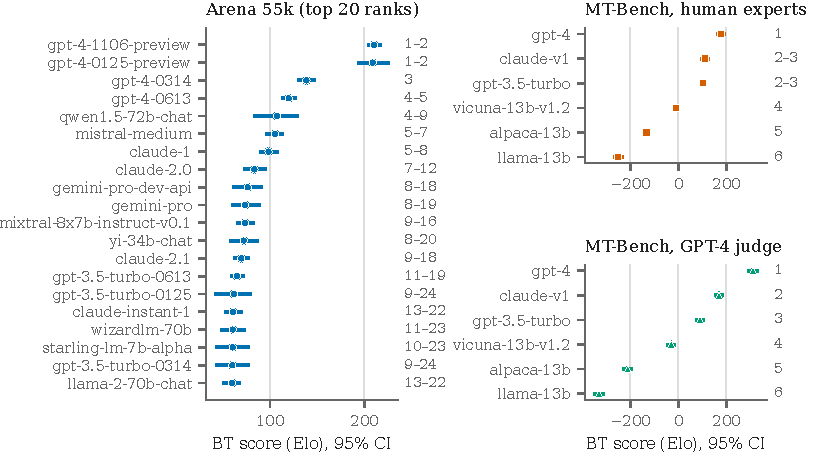
\includegraphics[width=\linewidth]{../figures/fig1_leaderboards.pdf}
\caption{Bradley--Terry scores (Elo scale) with 95\% bootstrap intervals ($B=1000$) and 95\% rank intervals; Arena 55k (ranks 1--20 of the 64-model fit) and MT-Bench (human experts, GPT-4 judge). Source: \texttt{results/base\_*.csv}.}
\label{fig:lb}
\end{figure}

\subsection{Results}
\paragraph{Resolved claims survive noise; unresolved ones do not.} Removing half of all comparisons at random leaves the top-1 claim intact with probability $\MTHRemConeHalf$ on MT-Bench human and $\MTGRemConeHalf$ on GPT-4, but only $\ArenaRemConeHalf$ on Arena and $\NBARemConeHalf$ on NBA all seasons; $\ArenaBootCone$ of Arena bootstrap resamples keep it (\texttt{results/random\_survival.csv}). Adjacent-pair claims are less stable: the share that hold in a bootstrap resample is $\ArenaBootCtwo$ (Arena), $\MTHBootCtwo$ (MT-Bench human), $\MTGBootCtwo$ (GPT-4) and $\NBABootCtwo$ (NBA all seasons), and removing 10\% of the comparisons keeps $\ArenaRemCtwoTen$, $\MTHRemCtwoTen$, $\MTGRemCtwoTen$ and $\NBARemCtwoTen$ of them. Figure~\ref{fig:surv} shows the survival curves with the verified adversarial budgets on the same axis.

\begin{figure}[t]
\centering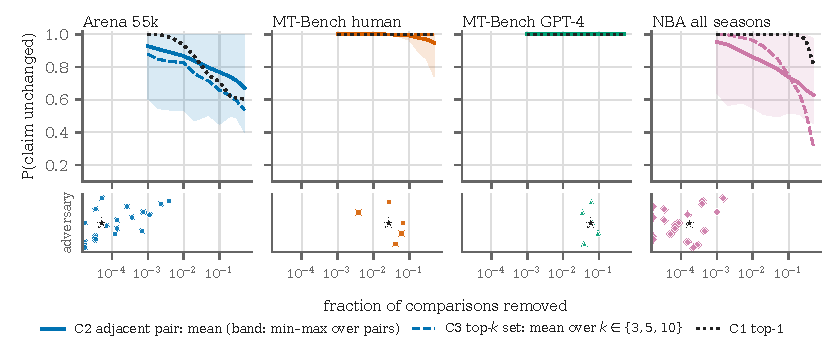
\includegraphics[width=\linewidth]{../figures/fig2_survival_remove.pdf}
\caption{Probability that a base-fit claim still holds after removing a random fraction $f$ of the comparisons (\nSeeds{} seeds per $f$): C1 (top-1), C2 (adjacent pairs; line: mean, band: min--max), C3 (top-$k$ set, mean over $k\in\{3,5,10\}$). Narrow panel: bootstrap resamples. Lower strip: verified adversarial removal budgets as a share of $N$, one marker per adjacent pair (rank 1 at the top), star: C1. Budgets are verified upper bounds.}
\label{fig:surv}
\end{figure}

\paragraph{The Arena top rank is a $\ArenaGapElo$-Elo margin; the resolved MT-Bench ranks take $2.7$--$6\%$ of the data.} The smallest verified set of removed comparisons that changes the top-1 claim has size $\ArenaConeB$ on Arena ($\ArenaConeFrac$ of $N=\ArenaN$; $z=\ArenaConeZ$; dataset-level 95\% interval \biArenaConeRange), $\MTHConeB$ on MT-Bench human ($\MTHConeFrac$ of $\MTHN$; $z=\MTHConeZ$; \biMTHConeRange) and $\MTGConeB$ on GPT-4 ($\MTGConeFrac$ of $\MTGN$; $z=\MTGConeZ$; \biMTGConeRange). On the $\nSeasons$ NBA seasons (about $\NBAsNgames$ games each) the median is $\NBAsConeMed$ games (maximum $\NBAsConeMax$); the NBA all-seasons ranking needs $\NBAConeB$ games (\biNBAConeRange). Removing the same $\ArenaConeB$ comparisons at random flips the Arena claim in $\ArenaRandFlipAtK$ of draws and no MT-Bench claim. The Arena budget is small because the data do not resolve the claim: random removal flips it with probability 5\% after $\nzArenaCone$ comparisons. Table~\ref{tab:head} summarises the budgets of all claims.

\begin{table}[t]
\caption{Verified adversarial removal budgets per dataset (exact ties excluded; upper bounds on the minimum), with dataset-level 95\% intervals (outward-rounded; resamples of all comparisons, 100--200, each searched anew; not available for the 69 NBA seasons). C1: top-1 claim; C2: adjacent-pair claims, median [min, max] in comparisons and median share of $N$; $z$: gap$/$bootstrap SE; ``\% of pair's comparisons'': median budget as a share of the comparisons involving either participant of the claim; verified: share of claims for which an exact refit confirmed the flip. On Arena and NBA all seasons the claims concern ranks 1--20 of the fit.}
\label{tab:head}
\centering\scriptsize
\resizebox{\linewidth}{!}{\begin{tabular}{lrccccccccc}
\toprule
 & Data & \multicolumn{2}{c}{C1 budget} & \multicolumn{3}{c}{C2 budget (comparisons)} & C2 median & median & C2 median, & \\
\cmidrule(lr){3-4}\cmidrule(lr){5-7}
Dataset & sets & count (\% of $N$) & 95\% interval & median & 95\% interval & min--max & \% of $N$ & $z$ iid / cluster & \% of pair's comparisons & verified \\
\midrule
Arena 55k & 1 & 3 (0.01\%) & [1, 50] & 7 & [4, 14] & 1--222 & 0.012\% & 0.25 / 0.25 & 0.1\% & 100\% \\
MT-Bench human & 1 & 91 (2.71\%) & [55, 128] & 141 & [113, 177] & 13--229 & 4.203\% & 7.87 / 5.60 & 7.2\% & 100\% \\
MT-Bench GPT-4 & 1 & 144 (6.00\%) & [105, 192] & 144 & [106, 169] & 82--226 & 6.000\% & 8.93 / 5.59 & 10.0\% & 100\% \\
NBA all seasons & 1 & 10 (0.02\%) & [1, 17] & 5 & [3, 11] & 1--90 & 0.008\% & 0.18 / 0.11 & 0.1\% & 100\% \\
NBA single seasons & 68 & median 4.5 (0.53\%) & -- & 2 & -- & 1--20 & 0.181\% & 0.23 / 0.24 & 1.2\% & 100\% \\
\bottomrule
\end{tabular}
}
\end{table}

\paragraph{Adjacent-rank claims are fragile when their margin is small, which is most of them outside MT-Bench.} The median budget of an adjacent-pair claim is $\ArenaCtwoMed$ comparisons on Arena (dataset-level interval \biArenaCtwoRange; $\ArenaCtwoFracMed$ of $N$), $\MTHCtwoMed$ (\biMTHCtwoRange) on MT-Bench human, $\MTGCtwoMed$ (\biMTGCtwoRange) on GPT-4, $\NBACtwoMed$ (\biNBACtwoRange) on NBA all seasons and $\NBAsCtwoMed$ games (inter-quartile range \NBAsCtwoQ) on an NBA season. Most of these claims are unresolved to begin with: the median $z$ is $\ArenaCtwoZMed$ on Arena and $\NBAsCtwoZMed$ on NBA seasons, where $\zshArenaIid$ and $\zshNBAsIid$ of the claims have $z<1$; the $\ArenaCtwoLowZ$ of $\ArenaCtwoCount$ Arena claims with $z<2$ need at most $\ArenaCtwoLowZBudMax$ removals. The i.i.d.\ bootstrap overstates $z$ where comparisons are clustered: the cluster bootstrap multiplies the SE by $\zshMTHSeRatio$ for MT-Bench human (clusters are questions) and $\zshNBASeRatio$ for NBA all seasons (seasons), lowering the median $z$ from $\zshMTHMedIid$ to $\zshMTHMedClu$ and from $\zshNBAMedIid$ to $\zshNBAMedClu$, and leaves Arena unchanged (ratio $\zshArenaSeRatio$; only identical prompts can be clustered). The conclusions do not change: MT-Bench claims remain resolved and most Arena and NBA claims do not. A flip at such margins needs no adversary; it is what a little noise does.

\paragraph{Budgets scale with the margin, as a first-order argument predicts, but the fitted line does not transfer.} To first order, removing a cell changes the gap $\theta_a-\theta_b$ by an amount fixed by the cell's influence, so closing a gap $g=z\cdot SE$ takes $k\approx g/\bar\imath$ removals, with $\bar\imath$ the mean influence of the selected cells; $\log k$ is therefore linear in $\log z$ with slope near one if $SE$ and $\bar\imath$ vary little. The regression is a check that the verified search behaves like this model, not an independent discovery. Across adjacent-pair claims the pooled slope is $\slopePool$ (cluster-bootstrap interval $\slopePoolCI$, $R^2=\rsqPool$, $\nregPool$ claims, dataset-specific intercepts) and $\slopeCluPool$ $\slopeCluPoolCI$ with the cluster-bootstrap margin; it is $\slopeArena$ $\slopeArenaCI$ on Arena and $\slopeNBAs$ $\slopeNBAsCI$ on NBA seasons, where budgets are a few games and the integer floor flattens the relation. The pooled fit is carried by the NBA seasons ($\nregNBAs$ of $\nregPool$ claims; Arena $\nregArena$, MT-Bench $\nregMTfit$), so the per-dataset slopes are the more direct evidence. We do not interpret the influence signal-to-noise ratio as a regressor: it is collinear with $\log z$ ($r=\collArena$ on Arena, $\collNBAs$ on NBA seasons).

Two tests show how far this goes (Fig.~\ref{fig:z}a and b). First, the line fitted on NBA seasons alone (slope $\oosSlope$ $\oosSlopeCI$) is unbiased on the seasons but under-predicts the budgets of other datasets: the mean of $\log k$ minus the prediction is $\oosArenaBias$ on Arena, $\oosMTHBias$ on MT-Bench human and $\oosMTGBias$ on GPT-4, i.e.\ budgets $\oosArenaFold\times$, $\oosMTHFold\times$ and $\oosMTGFold\times$ larger than predicted. The margin does not carry the dataset's scale, and since design is confounded with dataset identity we do not attribute the offsets to the evaluation design. Second, the parameter-free first-order estimate $\hat k$ needs no fit: its median ratio to the verified budget is $\oosArenaKhatMed$ on Arena, $\oosNBAsKhatMed$ on NBA seasons, $\oosMTHKhatMed$ on MT-Bench human and $\oosMTGKhatMed$ on GPT-4, and it is within a factor two for $\oosArenaKhatTwo$, $\oosNBAsKhatTwo$, $\oosMTHKhatTwo$ and $\oosMTGKhatTwo$ of the claims. The linearisation overestimates the budget on MT-Bench, where removals interact.

\begin{figure}[t]
\centering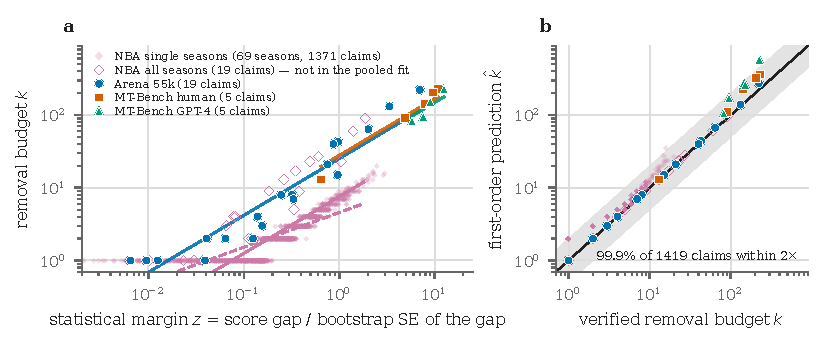
\includegraphics[width=\linewidth]{../figures/fig4_budget_vs_z.pdf}
\caption{Verified removal budget of each adjacent-pair claim against its margin $z$ (log--log). Solid lines: pooled fit $\log k=a_{\rm dataset}+b\log z$ (slope $\slopePool$, cluster-bootstrap 95\% interval $\slopePoolCI$); dashed: NBA seasons alone ($\slopeNBAs$ $\slopeNBAsCI$); Arena alone gives $\slopeArena$ $\slopeArenaCI$. Pooled NBA is plotted but not in the fit. Budgets are integers $\ge1$, hence the floor. (b) Parameter-free first-order estimate $\hat k$ against the verified budget; the band marks agreement within a factor two.}
\label{fig:z}
\end{figure}

\paragraph{A targeted set is $\nzNBAsRatio$--$\nzArenaRatio\times$ more effective than noise, and a rigger limited to its own target is nearly as effective as an unrestricted adversary.} The noise-equivalent budget of an adjacent-pair claim (median over claims) is $\nzArenaMed$ random removals on Arena, $\nzMTHMed$ on MT-Bench human, $\nzMTGMed$ on GPT-4, $\nzNBAMed$ on NBA all seasons and $\nzNBAsMed$ games on NBA seasons: $\nzArenaRatio$, $\nzMTHRatio$, $\nzMTGRatio$, $\nzNBARatio$ and $\nzNBAsRatio$ times the verified targeted budget. On MT-Bench human, random removal does not reach even a 5\% chance of flipping $\nzMTHNever$ of the claims. The constrained adversary needs a median of $\conArenaAdd$ added or $\conArenaRel$ relabelled comparisons on Arena (removal: $\ArenaCtwoMed$), $\conMTHAdd$ and $\conMTHRel$ on MT-Bench human ($\MTHCtwoMed$), $\conMTGAdd$ and $\conMTGRel$ on GPT-4 ($\MTGCtwoMed$), $\conNBAAdd$ and $\conNBARel$ on NBA all seasons ($\NBACtwoMed$) and $\conNBAsAdd$ and $\conNBAsRel$ on NBA seasons ($\NBAsCtwoMed$): $\conMTGRatioAdd$--$\conNBARatioAdd\times$ the removal budget for additions and $\conMTGRatioRel$--$\conArenaRatioRel\times$ for relabellings (Table~\ref{tab:add}; noise-equivalent budgets in Appendix Fig.~\ref{fig:noise}). The unconstrained adversary needs about as many additions as removals and about half as many relabellings. This is vote rigging \citep{min2025rigging} on a frozen snapshot; we do not simulate the platform's sampling or defences.

\begin{table}[t]
\caption{Verified budgets to reverse adjacent-pair claims by removing, adding or relabelling comparisons (medians over claims; ratio to removal as median [IQR]), unconstrained and constrained to the target (all added or relabelled comparisons involve the target). Noise-equivalent budgets: Fig.~\ref{fig:noise}.}
\label{tab:add}
\centering\scriptsize
\resizebox{\linewidth}{!}{\begin{tabular}{lrrrrccrrrrr}
\toprule
Data & Claims & \multicolumn{3}{c}{Median budget (comparisons)} & \multicolumn{2}{c}{Ratio to removal: median [IQR]} & \multicolumn{2}{c}{Constrained (median)} & \multicolumn{3}{c}{Random removals to flip (5\%)} \\
\cmidrule(lr){3-5}\cmidrule(lr){6-7}\cmidrule(lr){8-9}\cmidrule(lr){10-12}
 & & remove & add & relabel & add & relabel & add & relabel & median $k$ & never & $\div$ adversary \\
\midrule
Arena 55k & 19 & 7 & 6 & 4 & 1.00 [1.00, 1.00] & 0.57 [0.50, 0.88] & 8 & 7 & 1245 & 0\% & 198 \\
MT-Bench human & 5 & 141 & 134 & 67 & 0.95 [0.92, 0.99] & 0.50 [0.48, 0.51] & 173 & 137 & 2888 & 20\% & 31 \\
MT-Bench GPT-4 & 5 & 144 & 121 & 61 & 0.84 [0.80, 0.95] & 0.42 [0.40, 0.48] & 147 & 117 & 2111 & 0\% & 15 \\
NBA all seasons & 19 & 5 & 4 & 3 & 1.00 [1.00, 1.00] & 0.54 [0.50, 0.66] & 8 & 4 & 946 & 0\% & 118 \\
NBA single seasons & 1371 & 2 & 2 & 1 & 1.00 [1.00, 1.00] & 0.67 [0.50, 1.00] & 3 & 2 & 18 & 0\% & 9 \\
\bottomrule
\end{tabular}
}
\end{table}

\paragraph{Claims on the published output are cheaper to flip, and the estimator matters.} Only $\pubArenaSep$ of the $\pubArenaPairs$ adjacent Arena pairs are separated at base by the 95\% bootstrap interval ($\pubArenaSepShare$), against $\pubMTHSep$ of $\pubMTHPairs$ on MT-Bench human and $\pubMTGSep$ of $\pubMTGPairs$ on GPT-4. For these pairs the removal needed to make the re-bootstrapped interval include zero has a median of $\pubArenaBud$ comparisons on Arena (against $\pubArenaPoint$ for the same pairs' point gap to reverse), $\pubMTHBud$ on MT-Bench human ($\pubMTHPoint$) and $\pubMTGBud$ on GPT-4 ($\pubMTGPoint$): a claim of significance is cheaper to flip than a claim of order, by a factor of $1.3$--$2.9$. The claim that the top participant has rank interval $[1,1]$ holds at base on MT-Bench only (\pubMTHCprime{} and \pubMTGCprime{} claims; Arena: probability of rank 1 $\pubArenaPone$) and fails after $\pubMTHCprimeBud$ (human) and $\pubMTGCprimeBud$ (GPT-4) removals (Appendix Table~\ref{tab:pub}). The tie convention changes who is first: dropping ties makes \texttt{\estArenaDropTiesTop} the Arena top-1 model (Kendall $\tau=\estArenaDropTiesTau$ with the base ranking on the window) and moves the C1 budget from $\estArenaBaseCone$ to $\estArenaDropTiesCone$; counting a tie as one win and one loss gives $\estArenaTieWLCone$. On MT-Bench the C1 budget is $\estMTHDropTiesCone$ (human) and $\estMTGDropTiesCone$ (GPT-4) without ties, against $\estMTHBaseCone$ and $\estMTGBaseCone$. A practically unregularised fit ($\lambda=10^{-6}$) changes them by at most a few comparisons (Arena C1 $\estArenaUnregCone$, GPT-4 $\estMTGUnregCone$; Appendix Table~\ref{tab:est}).

\paragraph{Same questions, different labeller.} MT-Bench human and GPT-4 judgments agree on $\mtAgreeAll$ of the $3{,}355$ human judgments ($\mtAgreeNonTie$ when both are non-ties). Over the 15 model pairs, budgets under the two labellers are strongly rank-correlated (Spearman $\mtMASpB$ on the $\mtMAKeys$ keys the files share; $\mtMOSpB$ on the $\mtMOKeys$ keys that also match in presentation order), as are the $z$-gaps ($\mtMASpZ$, $\mtMOSpZ$), and the median ratio of GPT-4 to human budget is $\mtMARatioMed$ ($\mtMORatioMed$), range $\mtMARatioMin$--$\mtMARatioMax$ ($\mtMORatioMin$--$\mtMORatioMax$); the largest ratios belong to near-ties under human judgment. At equal participant set and size we find no evidence that the labeller changes fragility beyond its effect on the margin; with 15 pairs and one dataset per labeller the comparison has limited power (Appendix Fig.~\ref{fig:match}).

\paragraph{The search is verified and not beaten by exhaustive search or restarts.} Every budget above comes from an exact refit. A one-shot ranking of cells by influence is within $1.01\times$ everywhere, and the greedy search before polishing matches the final budget in all but $\mvUnpolImproved$ of $\mvUnpolN$ checked claims (Appendix Table~\ref{tab:valid}). On $\exInst$ random MT-Bench human subsamples (\exMs{} comparisons, six models) we enumerated all removal sets of up to $\exKmax$ comparisons for each of the $\exClaims$ adjacent-pair claims: the exact minimum was at most $\exKmax$ for $\exExactN$ claims, and the search with polishing returned exactly that minimum on $\exPolishEq$ of them (the unpolished greedy on $\exGreedyEqPct$, the one-shot ranking on $\exOneshotEqPct$); on the other $\exCensN$ claims no set of $\exKmax$ or fewer exists and the search returned $\exCensMinPolish$ or more. On the large instances we reran the search $\rsPer$ times per claim with random chunk sizes and noisy gain orders for $\rsClaims$ budget-defining pairs: no restart found a smaller set ($\rsBeat$ claims; $\rsAllEq$ of $\rsClaims$ identical, at most $\rsMaxRatio\times$ larger). This is evidence, not a certificate: the budgets of the main datasets remain upper bounds, and we have no lower bounds.

\paragraph{Controls: size, design and model structure.} \emph{Synthetic data} (labelled as such in \texttt{results/controls.csv}) with the real pair counts and tie shares and outcomes drawn from the BT model fitted to each real dataset give median budgets of $\ctlSynArenaB$ (real: $\ctlRealArenaB$), $\ctlSynMTHB$ ($\ctlRealMTHB$), $\ctlSynMTGB$ ($\ctlRealMTGB$) and $\ctlSynNBAB$ ($\ctlRealNBAB$) on Arena, MT-Bench human, GPT-4 and NBA all seasons, so the real budgets are close to what a well-specified BT model with the same counts predicts. \emph{N-matched subsampling} shows that size alone does not explain the datasets' differences: a random subsample of $3{,}355$ Arena comparisons (the size of MT-Bench human) has a median budget of $\ctlSubArenaMTHNB$ ($\ctlSubArenaMTHNFrac$ of $N$, median $z=\ctlSubArenaMTHNZ$), against $\ctlRealMTHB$ ($\ctlRealMTHFrac$) for MT-Bench human. Restricting Arena to the six MT-Bench models at $N=1{,}367$ gives a median share of $\ctlSixShare$ of $N$ over $\ctlSixDraws$ draws (95\% interval $\ctlSixLo$--$\ctlSixHi$), against $\ctlMTHSixShare$ ($\ctlMTHSixLo$--$\ctlMTHSixHi$) for $\ctlSixDraws$ MT-Bench human subsamples of the same size: a ratio of $\ctlSixRatio$ $\ctlSixRatioCI$. With five claims treated as independent draws the test detects a ratio of $\ctlSixMinDet$ or more, but only $\ctlSixMinDetClaim$ if claims are the unit, so the comparison shows no difference between labellers at equal participant set and size and does not bound one. The gap between Arena and MT-Bench is consistent with the participant set (64 models whose adjacent ranks differ by a fraction of a standard error, against six models separated by about eight) rather than with the number of comparisons or with crowd versus expert labels (Fig.~\ref{fig:ctl}).

\begin{figure}[t]
\centering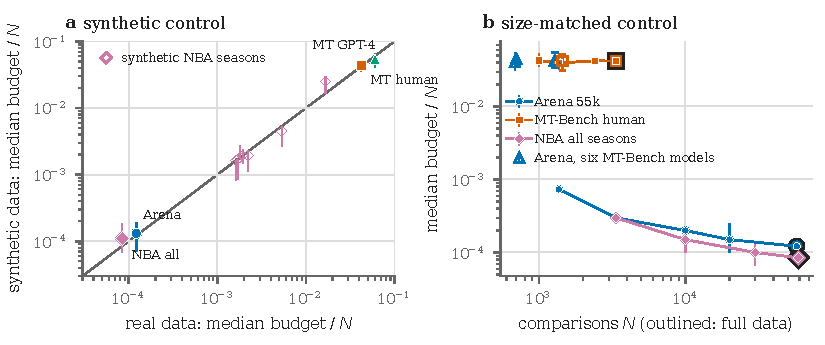
\includegraphics[width=\linewidth]{../figures/fig6_controls.pdf}
\caption{Controls (adjacent-pair claims, removal budgets, verified upper bounds). Synthetic data drawn from the BT fit of each real dataset with the real pair counts, and random subsamples at matched $N$ (Arena restricted to the six MT-Bench models, $\ctlSixDraws$ draws).}
\label{fig:ctl}
\end{figure}

\section{Discussion and Limitations}
\label{sec:limits}
\textbf{What the evidence says.} How sensitive a ranking claim is depends on how well the data resolve it. A resolved statement (large $z$, MT-Bench) survives noise and takes a targeted change of $\MTHConeFrac$--$\MTGConeFrac$ of the comparisons for the top rank, i.e.\ about a hundred comparisons, which a random perturbation of the same size does not do (and at least $\nzMTGRatio\times$ more random removals are needed). An unresolved statement (the Arena top rank at $\ArenaGapElo$ Elo, most adjacent Arena and NBA pairs) is fragile under the leaderboard's own bootstrap and flips after a handful of comparisons; reporting a rank without its margin hides this. Budgets grow with the margin, as first-order theory says, but how many comparisons a given margin costs depends on the dataset (a factor $\oosArenaFold$--$\oosMTHFold$ here), whereas the first-order estimate $\hat k$ tracks the budget without a fit. We see no sign of a labeller effect beyond the margin (limited power), and the controls make the number of comparisons an unlikely explanation of the Arena--MT-Bench difference. Evaluation design is confounded with dataset in our data (one crowd, one expert, one LLM-judge set, one sport), so we make no causal claim about design.

\textbf{Conditions of applicability.} The results are for BT scores fitted by $\ell_2$-regularised maximum likelihood ($\lambda=1$, ties as half a win) to frozen public snapshots, for claims defined relative to the base ranking and, on Arena and NBA all seasons, restricted to ranks 1--20 of the fit. Other estimators (online Elo, style-control covariates, anchoring) and platform filters may behave differently; of the choices we ablated, tie handling, the claim window and the claim type (point order versus published interval) change budgets by tens of per cent or more, and the ridge strength and home advantage do not.

\textbf{Limitations.} (1) Budgets are verified witnesses, hence upper bounds; we have no lower bounds, the exhaustive check covers budgets of up to five comparisons on six-model subsamples, and restarts are evidence, not proof. (2) The unconstrained adversary may delete or relabel any comparison; a real attacker controls only their own votes. The constrained adversary respects that but uses a proportional opponent allocation, not an optimised one, and ignores the platform's sampling, deduplication and defences. (3) The margins $z$ use an i.i.d.\ bootstrap; the cluster bootstrap changes them by up to $\zshNBASeRatio\times$ in the SE where clusters exist, and Arena has no usable cluster identifier. Claims within a dataset are not independent, and dataset-level intervals resample the comparisons of one snapshot, not the population of leaderboards. (4) The regressions rest on four datasets and are dominated by NBA seasons; the dataset offsets are descriptive. (5) The Arena--MT-Bench control has five claims per side. (6) The window of 20 is a convention. (7) The NBA all-seasons ranking mixes eras and is reported for reference only; NBA season budgets are a game or two and dominated by the integer floor. (8) Four datasets, one platform per design, no user or session identifiers.

\textbf{Broader impact.} Quantifying how few comparisons can change a ranking can help auditors decide which ranking statements to trust, and can also inform manipulation. We evaluate offline on frozen public data only and do not release tooling that interacts with a live platform.

\paragraph{LLM assistance disclosure.} The study, including planning, code, analysis and drafting of this paper, was carried out by AI agents based on Claude models, working in separate roles under the task's one-week CPU budget; the Bradley--Terry fits and all numbers come from the shipped code, not from a language model. An LLM-judge dataset (MT-Bench GPT-4 judgments) is itself one of the studied labelling designs. Reference lists were checked against the sources we consulted; the authors are responsible for every citation.

\bibliographystyle{plainnat}
\bibliography{references}

\appendix
\section{Additional results}
\FloatBarrier
\subsection{Claim window}
\label{app:window}
\IfFileExists{../figures/fig8_window.pdf}{Fig.~\ref{fig:win}}{The sweep} varies the window of claims on Arena and NBA all seasons. By score, the C1 budget on Arena is $\winArenaSTenCone$ for windows of 10, 20, 30, 40 and all 64 participants, because the runner-up is inside every window; the median adjacent budget is $\winArenaSTenCtwo$, $\winArenaSTwentyCtwo$, $\winArenaSThirtyCtwo$, $\winArenaSFortyCtwo$ and $\winArenaSAllCtwo$. By number of comparisons, the top-10, 20, 30 and 40 most-compared models give C1 budgets of $\winArenaCTenCone$, $\winArenaCTwentyCone$, $\winArenaCThirtyCone$ and $\winArenaCFortyCone$: the budget drops to $\winArenaCFortyCone$ only once the runner-up (rank 2, fewer comparisons than the 40th most compared model) enters the set. For NBA all seasons the C1 budget by score is $\winNBASTenCone$ for every window and the median adjacent budget $\winNBASTenCtwo$, $\winNBASTwentyCtwo$, $\winNBASThirtyCtwo$ and $\winNBASFortyCtwo$ for windows of 10, 20, 30 and 40. In the window of 20 by score, $\winArenaInside$ of all comparisons have both participants inside the window and $\winArenaTouch$ involve at least one; $\winArenaGeDirect$ of its 19 adjacent pairs have at least 100 direct comparisons. The window of 20 is thus a convention that keeps the adjacent pairs of the leaderboard's head, where the leaderboard's readers look, without excluding the runner-up.

\IfFileExists{../figures/fig8_window.pdf}{\begin{figure}[h]
\centering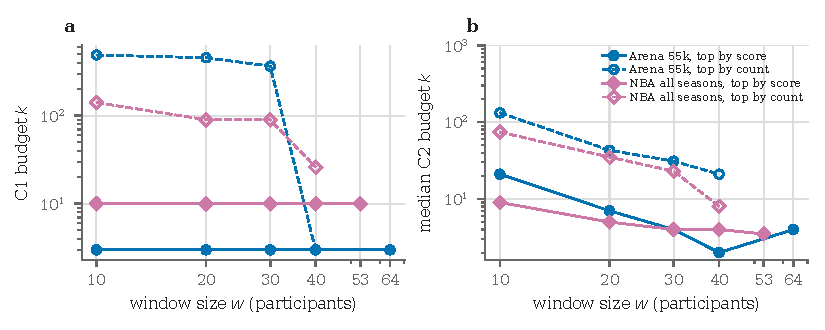
\includegraphics[width=\linewidth]{../figures/fig8_window.pdf}
\caption{Window sweep: C1 budget and median adjacent-pair budget against window size, for windows taken by score and by number of comparisons (Arena, NBA all seasons); the window used is marked.}
\label{fig:win}
\end{figure}}{}

\FloatBarrier
\subsection{Noise-equivalent budgets}
\begin{figure}[h]
\centering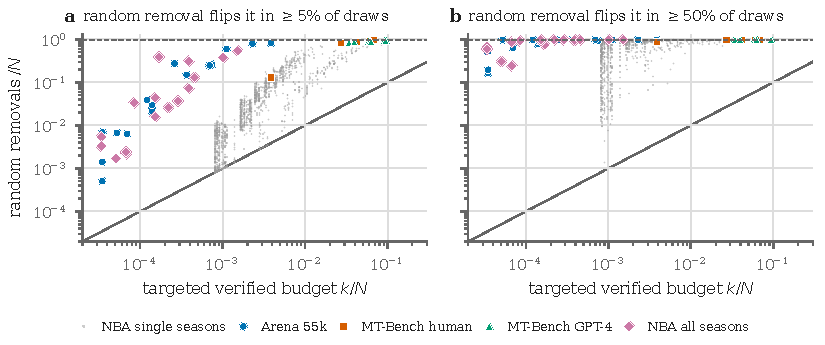
\includegraphics[width=\linewidth]{../figures/fig7_noise.pdf}
\caption{Targeted verified budget against the number of uniformly random removals that flips the same claim in at least 5\% (a) or 50\% (b) of 200 random draws (shares of $N$, log scales; claims C1 and adjacent pairs). Points on the dashed top line never reach that level by random removal. Diagonal: equal.}
\label{fig:noise}
\end{figure}

\FloatBarrier
\subsection{Per-rank budgets and regression}
\begin{figure}[h]
\centering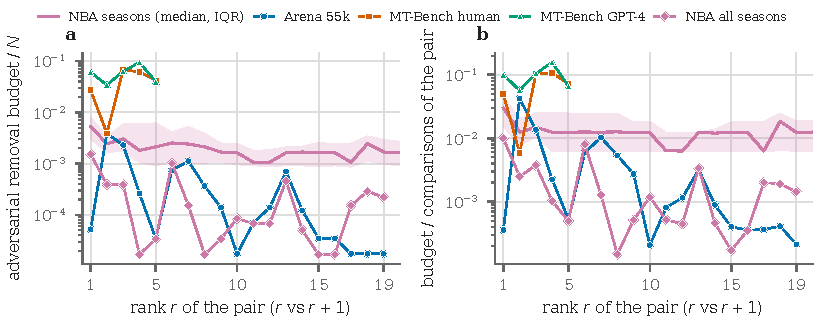
\includegraphics[width=\linewidth]{../figures/fig3_budgets.pdf}
\caption{Verified removal budgets of adjacent-pair claims by rank of the pair, per dataset (Arena: ranks 1--20 of the fit).}
\label{fig:rank}
\end{figure}
\begin{table}[h]
\caption{Regression of $\log k$ on $\log z$ with dataset-specific intercepts (cluster bootstrap by claim, stratified by dataset, $B=2000$). The signal-to-noise models are not reported: $\log z$ and $\log$ SNR are collinear (Section~\ref{sec:exp}).}
\label{tab:reg}
\centering\scriptsize
\resizebox{\linewidth}{!}{\begin{tabular}{llccrr}
\toprule
Fit & Model & slope on $\log z$ ($z_{\rm cl}$ in M0c, M1c) & $\log n_{\rm pair}$ & $R^2$ & claims \\
\midrule
Pooled, dataset intercepts & M0: $z$ & 0.78 [0.66, 0.85] & -- & 0.96 & 1400 \\
 & M1: $z$ + $n_{\rm pair}$ & 0.76 [0.62, 0.84] & 0.35 [$-$0.19, 0.93] & 0.96 & 1400 \\
 & M0c: $z_{\rm cl}$ & 0.77 [0.66, 0.84] & -- & 0.96 & 1400 \\
 & M1c: $z_{\rm cl}$ + $n_{\rm pair}$ & 0.75 [0.61, 0.82] & 0.41 [$-$0.13, 0.97] & 0.96 & 1400 \\
\midrule
NBA single seasons & M0: $z$ & 0.48 [0.44, 0.52] & -- & 0.71 & 1371 \\
 & M1: $z$ + $n_{\rm pair}$ & 0.48 [0.44, 0.52] & 0.19 [$-$0.08, 0.34] & 0.71 & 1371 \\
 & M0c: $z_{\rm cl}$ & 0.47 [0.44, 0.51] & -- & 0.70 & 1371 \\
 & M1c: $z_{\rm cl}$ + $n_{\rm pair}$ & 0.47 [0.44, 0.51] & 0.22 [$-$0.03, 0.39] & 0.70 & 1371 \\
\midrule
Arena 55k & M0: $z$ & 0.84 [0.69, 1.01] & -- & 0.91 & 19 \\
 & M1: $z$ + $n_{\rm pair}$ & 0.81 [0.63, 0.99] & 0.29 [$-$0.46, 0.94] & 0.92 & 19 \\
 & M0c: $z_{\rm cl}$ & 0.84 [0.69, 1.01] & -- & 0.91 & 19 \\
 & M1c: $z_{\rm cl}$ + $n_{\rm pair}$ & 0.81 [0.63, 1.00] & 0.29 [$-$0.45, 0.95] & 0.92 & 19 \\
\bottomrule
\end{tabular}
}
\end{table}

\FloatBarrier
\subsection{Search validity}
\begin{table}[h]
\caption{Verified budget of simpler heuristics relative to the final search (median, max over claims) and first-order estimate $\hat k$. Source: \texttt{results/method\_validity.csv}.}
\label{tab:valid}
\centering\scriptsize
\resizebox{\linewidth}{!}{\begin{tabular}{lrrrrrc}
\toprule
Method & Claims & Equal to best & Median ratio & 90th pct & Max & Verified \\
\midrule
Influence estimate (linearised, not refitted) & 48 & 65\% & 0.97 & 1.60 & 2.54 & no \\
One-shot influence ranking + exact refit & 48 & 98\% & 1.00 & 1.00 & 1.01 & yes \\
Greedy with exact refits & 48 & 98\% & 1.00 & 1.00 & 1.01 & yes \\
Greedy + swap/drop polish (used) & 48 & 100\% & 1.00 & 1.00 & 1.00 & yes \\
Heuristic: remove the pair's own decisive comparisons & 26 & 81\% & 1.00 & 1.13 & 1.50 & yes \\
Heuristic: remove the leader's wins & 47 & 9\% & 2.00 & 6.60 & 16.67 & yes \\
\bottomrule
\end{tabular}
}
\end{table}
\begin{table}[h]
\caption{Exhaustive search on small MT-Bench human subsamples: share of claims on which each search variant returns the exact minimum.}
\label{tab:exh}
\centering\scriptsize
\begin{tabular}{lrrrr}
\toprule
 & & \multicolumn{3}{c}{claims where the method returns the exact minimum} \\
\cmidrule(lr){3-5}
Claims grouped by & Claims & Greedy + polish (used) & Greedy, unpolished & One-shot ranking \\
\midrule
exact minimum 1 & 181 & 181 & 181 & 181 \\
exact minimum 2 & 149 & 149 & 148 & 148 \\
exact minimum 3 & 132 & 132 & 132 & 132 \\
exact minimum 4 & 105 & 105 & 105 & 103 \\
exact minimum 5 & 85 & 85 & 84 & 80 \\
\midrule
all with exact minimum $\le 5$ & 652 & 652 & 650 & 644 \\
no flip with $\le 5$ removals & 248 & 8 [6, 22] & 8 [6, 24] & 8.5 [6, 26] \\
\bottomrule
\end{tabular}

\end{table}
Restarts: $\rsPer$ randomised searches per claim for $\rsClaims$ budget-defining pairs found no smaller set than the deterministic search; $\rsAllEq$ matched it exactly and the largest restart/deterministic ratio is $\rsMaxRatio$.

\FloatBarrier
\subsection{Claims on the published output and estimator variants}
\begin{table}[h]
\caption{Left: share of adjacent pairs with margin $z<1$ under the i.i.d.\ bootstrap SE and a cluster bootstrap SE (clusters: MT-Bench question; Arena identical prompt text; NBA week, season for the all-seasons fit); SE ratio: median cluster$/$i.i.d. Right: the claim that the 95\% bootstrap interval of the score difference excludes 0: share of pairs for which it holds at base and, for those pairs, the median removal budget after which it fails when the perturbed data are re-bootstrapped, against the point-gap budget of the same pairs. C$_1^\prime$: the top participant has rank interval $[1,1]$ at base, and the median removal budget after which it fails.}
\label{tab:pub}
\centering\scriptsize
\resizebox{\linewidth}{!}{\begin{tabular}{lrrrcrrrrrr}
\toprule
 & \multicolumn{4}{c}{Margin: adjacent pairs with $z<1$} & \multicolumn{4}{c}{Claim: published 95\% intervals separate the pair} & \multicolumn{2}{c}{C1$^\prime$: top-1 rank interval is $[1,1]$} \\
\cmidrule(lr){2-5}\cmidrule(lr){6-9}\cmidrule(lr){10-11}
Dataset & Pairs & iid SE & cluster SE & SE ratio & Pairs & separated & median $k$, interval claim & $k$, same pairs, point gap & holds at base & median $k$ to fail \\
\midrule
Arena 55k & 19 & 84\% & 79\% & 0.98 & 19 & 16\% & 45 & 132 & 0/1 & -- \\
MT-Bench human & 5 & 20\% & 20\% & 1.73 & 5 & 80\% & 139.5 & 173 & 1/1 & 62 \\
MT-Bench GPT-4 & 5 & 0\% & 0\% & 1.70 & 5 & 100\% & 107 & 144 & 1/1 & 107 \\
NBA all seasons & 19 & 84\% & 100\% & 2.58 & 19 & 5\% & 14 & 90 & 0/1 & -- \\
NBA single seasons (right block: 7 sampled seasons) & 1371 & 94\% & 93\% & 0.98 & 151 & 2\% & 2 & 13 & 0/7 & -- \\
\bottomrule
\end{tabular}
}
\end{table}
\IfFileExists{../tables/table7_estimator.tex}{\begin{table}[h]
\caption{Estimator variants: C1 and median C2 budget, top-1 identity and Kendall $\tau$ on the claim window.}
\label{tab:est}
\centering\scriptsize
\resizebox{\linewidth}{!}{\begin{tabular}{llrclc}
\toprule
Data & Estimator & C1 budget & C2 median [min--max] & top-1 unchanged & Kendall $\tau$, window \\
\midrule
Arena 55k & baseline ($\lambda=1$, tie = half a win) & 3 & 7 [1--222] & yes & 1.00 \\
 & $\lambda=10^{-6}$ & 2 & 6 [1--225] & yes & 0.97 \\
 & ties removed & 6 & 6 [1--394] & no: gpt-4-0125-preview & 0.86 \\
 & tie = one win + one loss & 7 & 7 [1--197] & yes & 0.96 \\
\midrule
MT-Bench human & baseline ($\lambda=1$, tie = half a win) & 91 & 141 [13--229] & yes & 1.00 \\
 & $\lambda=10^{-6}$ & 91 & 141 [13--229] & yes & 1.00 \\
 & ties removed & 83 & 111 [7--198] & yes & 1.00 \\
 & tie = one win + one loss & 96 & 153 [16--244] & yes & 1.00 \\
\midrule
MT-Bench GPT-4 & baseline ($\lambda=1$, tie = half a win) & 144 & 144 [82--226] & yes & 1.00 \\
 & $\lambda=10^{-6}$ & 143 & 143 [82--225] & yes & 1.00 \\
 & ties removed & 77 & 83 [75--129] & yes & 1.00 \\
 & tie = one win + one loss & 153 & 148 [81--208] & yes & 1.00 \\
\midrule
NBA all seasons & baseline ($\lambda=1$, tie = half a win) & 10 & 5 [1--90] & yes & 1.00 \\
 & $\lambda=10^{-6}$ & 10 & 5 [1--89] & yes & 1.00 \\
\bottomrule
\end{tabular}
}
\end{table}}{}

\FloatBarrier
\subsection{Labeller comparison}
\begin{figure}[h]
\centering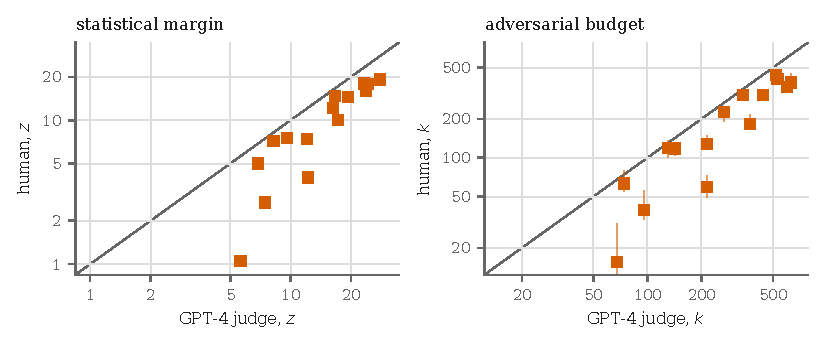
\includegraphics[width=\linewidth]{../figures/fig5_matched.pdf}
\caption{The 15 MT-Bench model pairs under two labellers at equal size ($N=1814$ matched keys). x: GPT-4 judge; y: one human judgment per key (median over 20 draws; bars: min--max). (a) margin $z$; (b) verified removal budget. Diagonal: equal.}
\label{fig:match}
\end{figure}

\FloatBarrier
\subsection{Ablation of modelling choices}
\begin{table}[h]
\caption{Median verified removal budget (comparisons) of the adjacent-pair claims under modelling variants; in brackets the 95\% percentile interval of the median budget as a \% of $N$ (claim-level bootstrap, $B=2000$; claims within a dataset are not independent, MT-Bench has five per judge). $\dagger$: median over all single-season claims with the home-advantage parameter, no interval available. ``--'': variant not run on that dataset. The Arena claim-set rows change the claim set and are not comparable claim by claim with the 19 baseline claims. Source: \texttt{results/ablations\_summary.csv}.}
\label{tab:abl}
\centering\scriptsize
\resizebox{\linewidth}{!}{\begin{tabular}{lccccc}
\toprule
Variant & Arena 55k & MT-Bench human & MT-Bench GPT-4 & NBA pooled & NBA single seasons \\
\midrule
Baseline ($\lambda=1$, ties = half a win) & 7 [0.0035, 0.037] & 141 [0.39, 6.8] & 144 [3.4, 9.4] & 5 [0.0034, 0.029] & 2 [0.17, 0.2] \\
Tied comparisons removed & 6 [0.0076, 0.045] & 111 [0.27, 7.7] & 83 [4.2, 7.2] & -- & -- \\
$\lambda=0.01$ & 6 [0.0052, 0.033] & 141 [0.39, 6.8] & 143 [3.4, 9.4] & 5 [0.0051, 0.029] & -- \\
$\lambda=100$ & 18 [0.007, 0.064] & 158 [0.27, 6.7] & 165 [3.5, 10] & 7 [0.0068, 0.022] & -- \\
Home-advantage parameter & -- & -- & -- & 5 [0.0051, 0.024] & 2$^\dagger$ \\
Playoff games added & -- & -- & -- & -- & 2 [0.17, 0.2] \\
Arena: window of 10 ranks & 21 [0.0052, 0.23] & -- & -- & -- & -- \\
Old claim set: 20 most-compared participants (Arena, NBA pooled) & 43 [0.043, 0.15] & -- & -- & 35 [0.039, 0.12] & -- \\
Arena: models with $\ge 1000$ comparisons (39 claims) & 21 [0.019, 0.054] & -- & -- & -- & -- \\
Arena: all 64 models (63 claims) & 4 [0.0035, 0.014] & -- & -- & -- & -- \\
\midrule
Claims (baseline) & 19 & 5 & 5 & 19 & 1371 \\
\bottomrule
\end{tabular}
}
\end{table}

\FloatBarrier
\section*{NeurIPS Paper Checklist}




\begin{enumerate}

\item {\bf Claims}
    \item[] Question: Do the main claims made in the abstract and introduction accurately reflect the paper's contributions and scope?
    \item[] Answer: \answerYes{} % Replace by \answerYes{}, \answerNo{}, or \answerNA{}.
    \item[] Justification: Abstract and introduction state the claims with their scope (four datasets, one estimator, claim windows, removal/addition/relabelling, no causal claim about design); results are in Section 4 and their limits in Section 5.
    \item[] Guidelines:
    \begin{itemize}
        \item The answer \answerNA{} means that the abstract and introduction do not include the claims made in the paper.
        \item The abstract and/or introduction should clearly state the claims made, including the contributions made in the paper and important assumptions and limitations. A \answerNo{} or \answerNA{} answer to this question will not be perceived well by the reviewers. 
        \item The claims made should match theoretical and experimental results, and reflect how much the results can be expected to generalize to other settings. 
        \item It is fine to include aspirational goals as motivation as long as it is clear that these goals are not attained by the paper. 
    \end{itemize}

\item {\bf Limitations}
    \item[] Question: Does the paper discuss the limitations of the work performed by the authors?
    \item[] Answer: \answerYes{} % Replace by \answerYes{}, \answerNo{}, or \answerNA{}.
    \item[] Justification: Section 5 lists the limitations and conditions of applicability.
    \item[] Guidelines:
    \begin{itemize}
        \item The answer \answerNA{} means that the paper has no limitation while the answer \answerNo{} means that the paper has limitations, but those are not discussed in the paper. 
        \item The authors are encouraged to create a separate ``Limitations'' section in their paper.
        \item The paper should point out any strong assumptions and how robust the results are to violations of these assumptions (e.g., independence assumptions, noiseless settings, model well-specification, asymptotic approximations only holding locally). The authors should reflect on how these assumptions might be violated in practice and what the implications would be.
        \item The authors should reflect on the scope of the claims made, e.g., if the approach was only tested on a few datasets or with a few runs. In general, empirical results often depend on implicit assumptions, which should be articulated.
        \item The authors should reflect on the factors that influence the performance of the approach. For example, a facial recognition algorithm may perform poorly when image resolution is low or images are taken in low lighting. Or a speech-to-text system might not be used reliably to provide closed captions for online lectures because it fails to handle technical jargon.
        \item The authors should discuss the computational efficiency of the proposed algorithms and how they scale with dataset size.
        \item If applicable, the authors should discuss possible limitations of their approach to address problems of privacy and fairness.
        \item While the authors might fear that complete honesty about limitations might be used by reviewers as grounds for rejection, a worse outcome might be that reviewers discover limitations that aren't acknowledged in the paper. The authors should use their best judgment and recognize that individual actions in favor of transparency play an important role in developing norms that preserve the integrity of the community. Reviewers will be specifically instructed to not penalize honesty concerning limitations.
    \end{itemize}

\item {\bf Theory assumptions and proofs}
    \item[] Question: For each theoretical result, does the paper provide the full set of assumptions and a complete (and correct) proof?
    \item[] Answer: \answerNA{} % Replace by \answerYes{}, \answerNo{}, or \answerNA{}.
    \item[] Justification: No theorems; the influence approximation is only used as a search heuristic and every budget is verified by exact refit.
    \item[] Guidelines:
    \begin{itemize}
        \item The answer \answerNA{} means that the paper does not include theoretical results. 
        \item All the theorems, formulas, and proofs in the paper should be numbered and cross-referenced.
        \item All assumptions should be clearly stated or referenced in the statement of any theorems.
        \item The proofs can either appear in the main paper or the supplemental material, but if they appear in the supplemental material, the authors are encouraged to provide a short proof sketch to provide intuition. 
        \item Inversely, any informal proof provided in the core of the paper should be complemented by formal proofs provided in appendix or supplemental material.
        \item Theorems and Lemmas that the proof relies upon should be properly referenced. 
    \end{itemize}

    \item {\bf Experimental result reproducibility}
    \item[] Question: Does the paper fully disclose all the information needed to reproduce the main experimental results of the paper to the extent that it affects the main claims and/or conclusions of the paper (regardless of whether the code and data are provided or not)?
    \item[] Answer: \answerYes{} % Replace by \answerYes{}, \answerNo{}, or \answerNA{}.
    \item[] Justification: Section 3 and the reproduction README give the estimator, claims, perturbations, seeds, data versions and checksums.
    \item[] Guidelines:
    \begin{itemize}
        \item The answer \answerNA{} means that the paper does not include experiments.
        \item If the paper includes experiments, a \answerNo{} answer to this question will not be perceived well by the reviewers: Making the paper reproducible is important, regardless of whether the code and data are provided or not.
        \item If the contribution is a dataset and\slash or model, the authors should describe the steps taken to make their results reproducible or verifiable. 
        \item Depending on the contribution, reproducibility can be accomplished in various ways. For example, if the contribution is a novel architecture, describing the architecture fully might suffice, or if the contribution is a specific model and empirical evaluation, it may be necessary to either make it possible for others to replicate the model with the same dataset, or provide access to the model. In general. releasing code and data is often one good way to accomplish this, but reproducibility can also be provided via detailed instructions for how to replicate the results, access to a hosted model (e.g., in the case of a large language model), releasing of a model checkpoint, or other means that are appropriate to the research performed.
        \item While NeurIPS does not require releasing code, the conference does require all submissions to provide some reasonable avenue for reproducibility, which may depend on the nature of the contribution. For example
        \begin{enumerate}
            \item If the contribution is primarily a new algorithm, the paper should make it clear how to reproduce that algorithm.
            \item If the contribution is primarily a new model architecture, the paper should describe the architecture clearly and fully.
            \item If the contribution is a new model (e.g., a large language model), then there should either be a way to access this model for reproducing the results or a way to reproduce the model (e.g., with an open-source dataset or instructions for how to construct the dataset).
            \item We recognize that reproducibility may be tricky in some cases, in which case authors are welcome to describe the particular way they provide for reproducibility. In the case of closed-source models, it may be that access to the model is limited in some way (e.g., to registered users), but it should be possible for other researchers to have some path to reproducing or verifying the results.
        \end{enumerate}
    \end{itemize}


\item {\bf Open access to data and code}
    \item[] Question: Does the paper provide open access to the data and code, with sufficient instructions to faithfully reproduce the main experimental results, as described in supplemental material?
    \item[] Answer: \answerYes{} % Replace by \answerYes{}, \answerNo{}, or \answerNA{}.
    \item[] Justification: Datasets are public with pinned versions and checksums; the code and scripts to regenerate every number are in the submission (anonymised); raw data are not redistributed.
    \item[] Guidelines:
    \begin{itemize}
        \item The answer \answerNA{} means that paper does not include experiments requiring code.
        \item Please see the NeurIPS code and data submission guidelines (\url{https://neurips.cc/public/guides/CodeSubmissionPolicy}) for more details.
        \item While we encourage the release of code and data, we understand that this might not be possible, so \answerNo{} is an acceptable answer. Papers cannot be rejected simply for not including code, unless this is central to the contribution (e.g., for a new open-source benchmark).
        \item The instructions should contain the exact command and environment needed to run to reproduce the results. See the NeurIPS code and data submission guidelines (\url{https://neurips.cc/public/guides/CodeSubmissionPolicy}) for more details.
        \item The authors should provide instructions on data access and preparation, including how to access the raw data, preprocessed data, intermediate data, and generated data, etc.
        \item The authors should provide scripts to reproduce all experimental results for the new proposed method and baselines. If only a subset of experiments are reproducible, they should state which ones are omitted from the script and why.
        \item At submission time, to preserve anonymity, the authors should release anonymized versions (if applicable).
        \item Providing as much information as possible in supplemental material (appended to the paper) is recommended, but including URLs to data and code is permitted.
    \end{itemize}


\item {\bf Experimental setting/details}
    \item[] Question: Does the paper specify all the training and test details (e.g., data splits, hyperparameters, how they were chosen, type of optimizer) necessary to understand the results?
    \item[] Answer: \answerNA{} % Replace by \answerYes{}, \answerNo{}, or \answerNA{}.
    \item[] Justification: No training; fitting details (ridge strength, tie handling, solver tolerance) are in Section 3 and the reproduction notes.
    \item[] Guidelines:
    \begin{itemize}
        \item The answer \answerNA{} means that the paper does not include experiments.
        \item The experimental setting should be presented in the core of the paper to a level of detail that is necessary to appreciate the results and make sense of them.
        \item The full details can be provided either with the code, in appendix, or as supplemental material.
    \end{itemize}

\item {\bf Experiment statistical significance}
    \item[] Question: Does the paper report error bars suitably and correctly defined or other appropriate information about the statistical significance of the experiments?
    \item[] Answer: \answerYes{} % Replace by \answerYes{}, \answerNo{}, or \answerNA{}.
    \item[] Justification: Seeds ($200$ per perturbation size), bootstrap ($B=1000$) and claim-level cluster-bootstrap intervals ($B=2000$) are reported; budgets carry dataset-level 95\% intervals from resampling the comparisons (100--200 resamples, each searched anew), and claim-level dependence is stated as a limitation. The control with five claims per side is flagged as underpowered.
    \item[] Guidelines:
    \begin{itemize}
        \item The answer \answerNA{} means that the paper does not include experiments.
        \item The authors should answer \answerYes{} if the results are accompanied by error bars, confidence intervals, or statistical significance tests, at least for the experiments that support the main claims of the paper.
        \item The factors of variability that the error bars are capturing should be clearly stated (for example, train/test split, initialization, random drawing of some parameter, or overall run with given experimental conditions).
        \item The method for calculating the error bars should be explained (closed form formula, call to a library function, bootstrap, etc.)
        \item The assumptions made should be given (e.g., Normally distributed errors).
        \item It should be clear whether the error bar is the standard deviation or the standard error of the mean.
        \item It is OK to report 1-sigma error bars, but one should state it. The authors should preferably report a 2-sigma error bar than state that they have a 96\% CI, if the hypothesis of Normality of errors is not verified.
        \item For asymmetric distributions, the authors should be careful not to show in tables or figures symmetric error bars that would yield results that are out of range (e.g., negative error rates).
        \item If error bars are reported in tables or plots, the authors should explain in the text how they were calculated and reference the corresponding figures or tables in the text.
    \end{itemize}

\item {\bf Experiments compute resources}
    \item[] Question: For each experiment, does the paper provide sufficient information on the computer resources (type of compute workers, memory, time of execution) needed to reproduce the experiments?
    \item[] Answer: \answerYes{} % Replace by \answerYes{}, \answerNo{}, or \answerNA{}.
    \item[] Justification: CPU only; measured wall times per step and the machine are in the reproduction notes (results/runtimes.csv).
    \item[] Guidelines:
    \begin{itemize}
        \item The answer \answerNA{} means that the paper does not include experiments.
        \item The paper should indicate the type of compute workers CPU or GPU, internal cluster, or cloud provider, including relevant memory and storage.
        \item The paper should provide the amount of compute required for each of the individual experimental runs as well as estimate the total compute. 
        \item The paper should disclose whether the full research project required more compute than the experiments reported in the paper (e.g., preliminary or failed experiments that didn't make it into the paper). 
    \end{itemize}
    
\item {\bf Code of ethics}
    \item[] Question: Does the research conducted in the paper conform, in every respect, with the NeurIPS Code of Ethics \url{https://neurips.cc/public/EthicsGuidelines}?
    \item[] Answer: \answerYes{} % Replace by \answerYes{}, \answerNo{}, or \answerNA{}.
    \item[] Justification: The work uses only public data, no human subjects, and we discuss misuse in Section 5.
    \item[] Guidelines:
    \begin{itemize}
        \item The answer \answerNA{} means that the authors have not reviewed the NeurIPS Code of Ethics.
        \item If the authors answer \answerNo, they should explain the special circumstances that require a deviation from the Code of Ethics.
        \item The authors should make sure to preserve anonymity (e.g., if there is a special consideration due to laws or regulations in their jurisdiction).
    \end{itemize}


\item {\bf Broader impacts}
    \item[] Question: Does the paper discuss both potential positive societal impacts and negative societal impacts of the work performed?
    \item[] Answer: \answerYes{} % Replace by \answerYes{}, \answerNo{}, or \answerNA{}.
    \item[] Justification: Section 5 (Broader impact) discusses auditing benefits and manipulation risks.
    \item[] Guidelines:
    \begin{itemize}
        \item The answer \answerNA{} means that there is no societal impact of the work performed.
        \item If the authors answer \answerNA{} or \answerNo, they should explain why their work has no societal impact or why the paper does not address societal impact.
        \item Examples of negative societal impacts include potential malicious or unintended uses (e.g., disinformation, generating fake profiles, surveillance), fairness considerations (e.g., deployment of technologies that could make decisions that unfairly impact specific groups), privacy considerations, and security considerations.
        \item The conference expects that many papers will be foundational research and not tied to particular applications, let alone deployments. However, if there is a direct path to any negative applications, the authors should point it out. For example, it is legitimate to point out that an improvement in the quality of generative models could be used to generate Deepfakes for disinformation. On the other hand, it is not needed to point out that a generic algorithm for optimizing neural networks could enable people to train models that generate Deepfakes faster.
        \item The authors should consider possible harms that could arise when the technology is being used as intended and functioning correctly, harms that could arise when the technology is being used as intended but gives incorrect results, and harms following from (intentional or unintentional) misuse of the technology.
        \item If there are negative societal impacts, the authors could also discuss possible mitigation strategies (e.g., gated release of models, providing defenses in addition to attacks, mechanisms for monitoring misuse, mechanisms to monitor how a system learns from feedback over time, improving the efficiency and accessibility of ML).
    \end{itemize}
    
\item {\bf Safeguards}
    \item[] Question: Does the paper describe safeguards that have been put in place for responsible release of data or models that have a high risk for misuse (e.g., pre-trained language models, image generators, or scraped datasets)?
    \item[] Answer: \answerNA{} % Replace by \answerYes{}, \answerNo{}, or \answerNA{}.
    \item[] Justification: No model or dataset with high misuse risk is released; the analysis is offline on frozen data.
    \item[] Guidelines:
    \begin{itemize}
        \item The answer \answerNA{} means that the paper poses no such risks.
        \item Released models that have a high risk for misuse or dual-use should be released with necessary safeguards to allow for controlled use of the model, for example by requiring that users adhere to usage guidelines or restrictions to access the model or implementing safety filters. 
        \item Datasets that have been scraped from the Internet could pose safety risks. The authors should describe how they avoided releasing unsafe images.
        \item We recognize that providing effective safeguards is challenging, and many papers do not require this, but we encourage authors to take this into account and make a best faith effort.
    \end{itemize}

\item {\bf Licenses for existing assets}
    \item[] Question: Are the creators or original owners of assets (e.g., code, data, models), used in the paper, properly credited and are the license and terms of use explicitly mentioned and properly respected?
    \item[] Answer: \answerYes{} % Replace by \answerYes{}, \answerNo{}, or \answerNA{}.
    \item[] Justification: All datasets are cited with versions and licences in the reproduction notes (apache-2.0, cc-by-4.0, CC-BY-4.0); no dataset without declared licence is used.
    \item[] Guidelines:
    \begin{itemize}
        \item The answer \answerNA{} means that the paper does not use existing assets.
        \item The authors should cite the original paper that produced the code package or dataset.
        \item The authors should state which version of the asset is used and, if possible, include a URL.
        \item The name of the license (e.g., CC-BY 4.0) should be included for each asset.
        \item For scraped data from a particular source (e.g., website), the copyright and terms of service of that source should be provided.
        \item If assets are released, the license, copyright information, and terms of use in the package should be provided. For popular datasets, \url{paperswithcode.com/datasets} has curated licenses for some datasets. Their licensing guide can help determine the license of a dataset.
        \item For existing datasets that are re-packaged, both the original license and the license of the derived asset (if it has changed) should be provided.
        \item If this information is not available online, the authors are encouraged to reach out to the asset's creators.
    \end{itemize}

\item {\bf New assets}
    \item[] Question: Are new assets introduced in the paper well documented and is the documentation provided alongside the assets?
    \item[] Answer: \answerYes{} % Replace by \answerYes{}, \answerNo{}, or \answerNA{}.
    \item[] Justification: The derived result tables and code are documented in results/README.md and code/REPRODUCE.md.
    \item[] Guidelines:
    \begin{itemize}
        \item The answer \answerNA{} means that the paper does not release new assets.
        \item Researchers should communicate the details of the dataset\slash code\slash model as part of their submissions via structured templates. This includes details about training, license, limitations, etc. 
        \item The paper should discuss whether and how consent was obtained from people whose asset is used.
        \item At submission time, remember to anonymize your assets (if applicable). You can either create an anonymized URL or include an anonymized zip file.
    \end{itemize}

\item {\bf Crowdsourcing and research with human subjects}
    \item[] Question: For crowdsourcing experiments and research with human subjects, does the paper include the full text of instructions given to participants and screenshots, if applicable, as well as details about compensation (if any)? 
    \item[] Answer: \answerNA{} % Replace by \answerYes{}, \answerNo{}, or \answerNA{}.
    \item[] Justification: No crowdsourcing was performed; existing public votes were reanalysed.
    \item[] Guidelines:
    \begin{itemize}
        \item The answer \answerNA{} means that the paper does not involve crowdsourcing nor research with human subjects.
        \item Including this information in the supplemental material is fine, but if the main contribution of the paper involves human subjects, then as much detail as possible should be included in the main paper. 
        \item According to the NeurIPS Code of Ethics, workers involved in data collection, curation, or other labor should be paid at least the minimum wage in the country of the data collector. 
    \end{itemize}

\item {\bf Institutional review board (IRB) approvals or equivalent for research with human subjects}
    \item[] Question: Does the paper describe potential risks incurred by study participants, whether such risks were disclosed to the subjects, and whether Institutional Review Board (IRB) approvals (or an equivalent approval/review based on the requirements of your country or institution) were obtained?
    \item[] Answer: \answerNA{} % Replace by \answerYes{}, \answerNo{}, or \answerNA{}.
    \item[] Justification: No new human-subject research; only existing public data were used.
    \item[] Guidelines:
    \begin{itemize}
        \item The answer \answerNA{} means that the paper does not involve crowdsourcing nor research with human subjects.
        \item Depending on the country in which research is conducted, IRB approval (or equivalent) may be required for any human subjects research. If you obtained IRB approval, you should clearly state this in the paper. 
        \item We recognize that the procedures for this may vary significantly between institutions and locations, and we expect authors to adhere to the NeurIPS Code of Ethics and the guidelines for their institution. 
        \item For initial submissions, do not include any information that would break anonymity (if applicable), such as the institution conducting the review.
    \end{itemize}

\item {\bf Declaration of LLM usage}
    \item[] Question: Does the paper describe the usage of LLMs if it is an important, original, or non-standard component of the core methods in this research? Note that if the LLM is used only for writing, editing, or formatting purposes and does \emph{not} impact the core methodology, scientific rigor, or originality of the research, declaration is not required.
    %this research? 
    \item[] Answer: \answerYes{} % Replace by \answerYes{}, \answerNo{}, or \answerNA{}.
    \item[] Justification: LLM assistance in planning, coding and writing is disclosed in Section 5; no LLM is part of the method except that MT-Bench GPT-4 judgments are one analysed dataset.
    \item[] Guidelines:
    \begin{itemize}
        \item The answer \answerNA{} means that the core method development in this research does not involve LLMs as any important, original, or non-standard components.
        \item Please refer to our LLM policy in the NeurIPS handbook for what should or should not be described.
    \end{itemize}

\end{enumerate}
\end{document}
